\documentclass{article}
\usepackage[utf8]{inputenc}
\usepackage{amsmath}
\usepackage{graphicx}
\usepackage[margin=1.5in]{geometry}
\usepackage{float}
\setlength{\parindent}{0pt}


\title{TA manual Motion Analysis}
\author{Joris Busink}
\date{May 2023}

\begin{document}

\maketitle

\tableofcontents

\newpage

\section{Introduction}
This manual is designed to assist Teacher Assistants (TA's) in effectively teaching the Motion Analysis (MA) experiment to second-year bachelor students in the MNW2 practical and NSP2 practical series. This manual aims to provide detailed guidance on essential aspects, including proficient handling of scientific equipment, implementing an optimal data acquisition strategy and we present several example experiments that the students can study within the given time constraint. The first part of the manual was originally written by Munib Ozdemir as part of an education project. It was translated and adapted in this manual. We value your input and suggestions to enhance this manual further.

\newpage 

\section{Hardware \& software}
In this section, we will provide an overview of the scientific equipment utilized in the MA experiment, along with technical details and helpful tips and tricks for both students and TA's. For a more comprehensive understanding of the hardware, we direct readers to the student manual. While these camera fundamentals may appear elementary to some, it is worth noting that students generally have limited prior experience with cameras and photography. 

\subsection{Hardware: Camera and zoom lens}
During the MA experiment, students will use the Lumenera Lt225C high-speed camera to capture a dynamical process. The camera features a 2/3 inch CMOS sensor with a resolution of 2048x1088 pixels and has a fully Electronic Global Shutter, it will capture an image by turning all the pixels on and off electronically. The camera is capable of recording at approximately 700 frames per second (fps), but this depends on the resolution and color depth of the image. The image is displayed on the camera using an already affixed zoom lens. The zoom lens consists of three components (from left to right): $1)$ a focus ring, 2$)$ a zoom ring and $3)$ an aperture ring. The function of each of these elements is the following:

\begin{itemize}
    \item Aperture (ring): the aperture refers to the adjustable opening in the camera lens that controls the amount of light entering the camera. It is often represented by the f-number, such as f/2.8, f/4, f/5.6, and so on. The f-number is the ratio of focal length f to the effective aperture diameter D, with symbol N. $N = f/D$. The numbers ($\textbf{ranging from 1.4 to 22}$) on the aperature ring provide the f-number ($\textbf{symbol N, excersise 1}$). The aperture plays a vital role in the MA experiment as it influences two main aspects: the exposure and the depth of field.
    Regarding depth of field, the aperture size affects the range of distances that appear in sharp focus within an image. A wider aperture (lower f-number) creates a shallow depth of field, i.e. the background appears blurred. On the other hand, a narrower aperture (higher f-number) increases the depth of field.

    \item Zoom ring: a zoom ring is a control ring on a camera or lens that allows you to adjust the focal length  ($\textbf{symbol f, excersise 1}$), enabling you to zoom in or out and control the magnification and field of view of the captured image. The focal length of the camera is second list of engraved marking, $\textbf{ranging from 11.5 to 69 mm}$. 
    
    \item focus (ring): the focus ring in a camera is a manual control mechanism located on the camera lens. It allows the user to manually adjust the focal distance of the lens. By rotating the focus ring, the lens elements move back and forth, altering the focal length. This allows the user to bring the object into sharp focus. A sharp focus allows to study finer details of the motion of the dynamical process.
        
\end{itemize}

Besides the terminology of the camera and zoom-lens, students will also encounter some terminology regarding the data-acquisition. This includes concepts such as frame rate, depth of field, color depth, and more, may be unfamiliar to them. Therefore, it is the TA's responsibility to acquaint the students with these terms and provide practical guidance on their utilization throughout the experiment. 

The list below shows common terminology used in the MA experiment. It is important to, not only, understand the terminology, but also to use it correctly in the experiments. A good understanding of the terminology and concepts saves a tremendous amount of time in the processing of the data! 

\begin{itemize}
    \item Plane of focus: the plane of focus is the distance in the scene where objects appear sharpest and in focus when captured by the camera.
    
    \item Depth of Field (Dof): the distance between the nearest and the farthest objects that are in acceptably sharp focus in an image captured with a camera. The precise definition of "sharp focus" is subjective, as it relies on individual perception. Nonetheless, an empirical understanding of DoF can be gained through an experiment using a paper with a basic text message. By manipulating the camera's focus to capture the text and observing the resultant image, one can establish the boundaries of the DoF. By systematically adjusting the position of the paper, an intuitive sense of optimal focus can be developed. The DoF is quantified by the extent of the range between the closest and farthest objects that results in a sharp focus. 
    
    \item Circle of confusion (CoC): the circle of confusion, denoted by c, is the maximum allowable blur circle size that still appears as a sharp point in an image. It depends on the sensor size, lens characteristics, aperture setting, and viewing conditions. In the experiment we will use a static value of c = 0.008 $10^{-3}$m. Students may ask questions about the CoC, you can refer them to a quick google (image) search. It is a rather technical term that is difficult to explain and we do not use it any further in the experiments, apart from the introduction experiment ($\textbf{excersise 1}$).
    
    \item Frames per second (fps): Frames per second (fps) refers to the number of frames or images the camera can capture per second, equivalent to the framerate. While the term may seem self-explanatory, it is crucial to optimize the fps setting during the experiment. Although the Lumenera Lt225C camera can reach a maximum of approximately 700 fps (and even higher if desired), it is important to consider the limitations of the hardware's data acquisition rate. When working with high-resolution settings, the hardware's bandwidth becomes the critical limiting factor. Futher note that a high fps results in a low amount of light collected on the CMOS chip. The image can becomes very dark and the lighting needs modification!

    To ensure efficient data collection, it is advisable to align the fps with the timescale of the experiment. For example, let's consider a mathematical pendulum with a length of 1 meter. Its period, denoted as T, can be calculated using the formula $T = 2\pi \sqrt{1/9.81} \approx 2$ seconds. If our aim is to capture 50 frames per swing, it is sufficient to limit ourselves to 25 fps. By doing so, we significantly reduce the amount of time required for data analysis, compared to capturing at the maximum 700 fps.
    
    By carefully selecting an appropriate fps setting that balances data acquisition needs with practical considerations, we can optimize the efficiency of the experiment and streamline subsequent data analysis efforts. 

    \item Pixel: picture element that is the smallest addressable element in a raster image. A pixel can be on or off (1 bit per pixel, 1 bpp) or have multiple colors e.g. 8bpp = 256 colours.
    
    \item Resolution: the resolution refers to the level of detail and clarity in an image or display. It is commonly expressed in terms of the number of pixels (picture elements) that make up the image, typically presented as width x height (e.g., 1920 x 1080 pixels). A higher resolution corresponds to a greater number of pixels, resulting in finer details and enhanced visual fidelity. However, it is essential to consider whether these additional details are necessary for the specific analysis at hand. In cases where fine-grained details are not crucial, opting for a lower resolution can be advantageous, as it reduces the volume of data to be processed. This can significantly streamline the data-processing workflow. The maximum resolution of the camera is 2048x1088 = 2228224 bits (or 0.278528 MB). This specification provides an estimation of the amount of data required to store each frame at maximum resolution, note that this is not the equivalent to the data stored on e.g. a harddrive.

    \item Colour Depth: the Chrominance/Luminance information per pixel. 
    For tracking we use typically 8bpp grayscale, so we have $2^8 = 256$ gray tones. 
    \item Bitrate: the number of bits that are processed per unit of time, e.g. 1 kbit/s = 1000 bits per second.
    The bitrate of the camera is the product of the resolution, the framerate and the colordepth. 
    For a given resolution of 2048x1088, at a framerate of 50 hz and a colordepth of 8bpp we have 111,669,760 bits per second! That is 111.67 MB per second. A typical USB2 port has a bandwidth of around 50 MB per second. So we cannot use these in this scenario.
    \item Bandwidth: maximum rate of data transfer across a given path. The cameras need to be connected to an USB3.0 port (or higher).
\end{itemize}


By controlling the aperture, zoom ring and/or the focus ring, and by optimizing the frame rate, resolution, etc. the students can optimize the raw footage of the dynamical process. It can take several attempts to create an optimized image-sequence, it is part of the experiment and should not be skipped at any point. An un-optimized image-sequence is very hard to analyze. It is therefore essential that the raw footage of the dynamical process is optimized. The students may use different lamps, supports, etc. to optimize their footage, be creative!


\subsection{Tips and tricks}

\begin{itemize}
    \item Use LED lights, black/white cardboard, theater lights to optimize contrast. 
    \item Use clamps to create a stable configuration. It is possible to rotate the camera by 90 (or any amount) degrees to create a canvas of 1088x2048 (instead of 2048x1088). You can correct the data during the data-processing. 
    \item Choose a framerate that is comparable to the timescale of the dynamical process.
    \item Use a resolution that captures the \emph{essential} details of the experiment. It is often more efficient to use a smaller resolution, since the data processing is much faster. In almost all cases, the limiting factor of an experiment is not the resolution.
    \item Before you make several movies, do a single analysis from start to finish. This avoids wasting time analyzing un-optimized footage.
\end{itemize}

\subsection{Software}
The software that is used during the experiment is the following:
\begin{itemize}
\item \textbf{LuCam Capture}. LuCam Capture is a very basic software to test the camera. LuCam Capture can only capture images, hence it cannot be used to make a movie. However, LuCam Capture is easy to use, and you can check the camera options and play around with them.
\item \textbf{TroublePix}. The video capturing is done with TroublePix. You can use the same camera options as LuCam Capture. You can change the camera settings in \emph{view}. Using TroublePix is straightforward and the settings can be found in the student manual.
To install the software on a new computer, please contact Gerrit Kuik. 
\item \textbf{MaxTRAQ}. Lastly, we use MaxTRAQ software. MaxTRAQ is the motion-analysis software that we will use. MaxTRAQ is able to track the position of points, the angle between the points, distances, etc. MaxTRAQ tracks objects by fitting an ellipsoid to the object of interest, the centre of the ellipsoid is the mean-position, thus the coordinates of objects. Furthermore, MaxTRAQ estimates, based on several frames, the velocity and the direction of the object, this enables us to track multiple objects without assignment problems (a very typical problem in multiple object tracking is that the software cannot distinguish the individual objects, this results in a messy data file.). To enable tracking, the object of interest needs to have a high contrast with respect to the background. Furthermore, the object needs to have a well-defined shape (e.g. circle, square, etc.). The shape of the object may vary between frames but it should not vanish or break-up between the frames. To optimize the shape of the object you can use LED lights, clamps, theater lights and markers.

At the start of the tracking analysis you have to select the objects to track. To track multiple object or when tracking angles, you have to select the appropriate settings and select each of the objects. For small objects, it can be useful to adjust the tracking region and sensitivity in the settings page. Before you track a whole video, try if you can see if the object is fully visible in the time-region of interest. If the object vanishes a lot it is most likely not worth investing the time to manually track every frame; you should make a better video. If the object is fully visible and does not break up, you can start the tracking software. The exact details to track the object are provided in the student manual. 

If the tracking fails, you can manually continue the tracking by re-selecting the (missed) object. If you have a very difficult object to track you can do the following things: 1$)$ make a better video, 2$)$ scroll with you mouse and select the missed objects during tracking (scrolling is much faster than checking the frames frame to frame.). Every time the tracking fails MaxTRAQ will pause the program. In the bottom graphs you can see the results of the object tracking (s-t, v-t or a-t).
\end{itemize}

\newpage

\section{Introduction experiment: Simple Pendulum}
\begin{figure}[H]
    \centering
    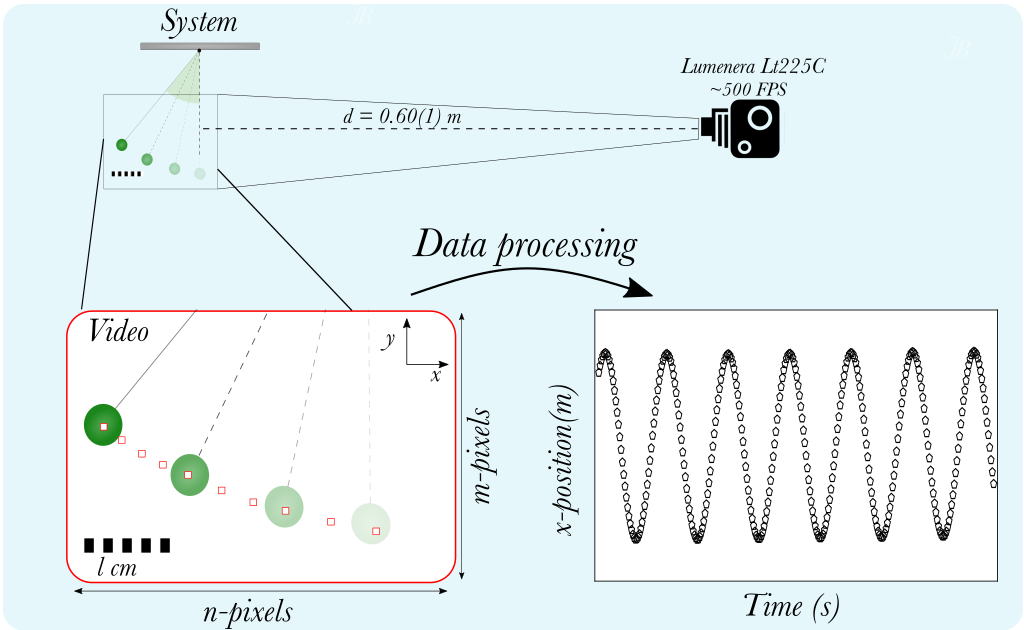
\includegraphics[width=12cm]{figures/Pendulum setup.png}
    \caption{The setup of the pendulum experiment. The LumeneraLi255C captures the motion of the simple pendulum. The x-position of the mass of the pendulum is tracked using MaxTRAQ, the resulting oscillatory movement is shown in the right bottom of the graph.}
    \label{Figure: Pendulum setup}
\end{figure}
\subsubsection{Theory}
The simple (mathematical) pendulum consists of a mass $m$ attached to a massless cord of length $l$. The mass is constrained to move in the azimuthal direction $\theta$ and cannot stretch $\dot{l}=0$. When the mass is pulled out of equilibrium at an angle $\theta$ it wil make an arc of length s, the net force it will experience is a gravitation force $F_g = -mg\sin{\theta}$. Hence, Newton's equation for the movement along the arc s is given by:

\begin{align}
    m\ddot{s} = -mg\sin(\theta).
\end{align}
The relationship between the arc length s and the angle $\theta$ is $s=l\theta$. The acceleration in the displacement direction s is therefore
\begin{align}
    ml\ddot{\theta} = -mg\sin{\theta} & \\
    \ddot{\theta} = -\omega_0^2\sin(\theta).
    \label{Eq. Pendulum}
\end{align}
Here we defined the angular (eigen)frequency $\omega_0^2 = g/l$. Eq. \ref{Eq. Pendulum} has no analytic solution for arbitrary angle $\theta$ (the solutions are of the form of elliptic integrals). But, for a small angle $\theta \approx 0$, we can Taylor expand the sinusoidal equation $\sin(\theta)\approx \theta$ and we arrive to 
\begin{align}
    \ddot{\theta} + \omega_0^2 \theta = 0.
    \label{Eq. Pendulum linear}
\end{align}
The solution of Eq. \ref{Eq. Pendulum linear} is an oscillation, hence 
\begin{align}
    \theta(t) = \theta_0\cos(\omega_0 t + \phi_0).
\end{align}
$\theta_0$ is the amplitude of the oscillation and $\phi_0$ is an arbitrary phase. 
If we choose the x-axis along the displacement axis, with $x = l\theta$ we arrive to:
\begin{align}
    x(t) = x_0\cos(\omega_0 t + \phi_0).
\end{align}
The period T is straightforward derived from the eigenfrequency

\begin{align}
    T=\frac{2\pi}{\omega}.
\end{align}

\subsubsection{Setup and results}
The mathematical pendulum experiment is offered in the introduction of the Motion Analysis experiment. The students should be able to build the experiment from scratch using the simple tools that are available in the practical room. The setup consist of a cord with length l with a mass m at the end. The linear frequency $\omega_0 = \sqrt{g/l}$, can be altered by varying the length of the cord. In Fig. \ref{Figure: Pendulum setup} the setup is shown. The setup does not offer a lot of freedom in adjusting the parameters, but the analysis can be extended. To track the motion of mass of the pendulum is relatively straightforward. By connecting a simple LED light to the cord it is possible to track the x-position and y-position. 

Although this experiment is offered as an introduction experiment, it is possible to investigate different pendulum experiments as a main experiment. A few example experiments can be done using this setup:

\subsubsection{Gravitational acceleration (easy)}
Calculate the gravitational acceleration g using the pendulum model. 
\begin{align}
    \omega_0 =\sqrt{\frac{g}{l}}
\end{align}
Students can calculate the gravitational acceleration by fitting the oscillator model to the x-direction of the pendulum. A possible extension is to use different lengths of the cord l and linearize the data. A more robust approach to calculate the gravitational acceleration is to include a third order term in the Taylor expansion (or even more) $\sin(\theta)\approx\theta - \frac{1}{6}\theta^3 +\dots$ and solve the equation. The resulting period depends on the angle of release an can be derived using a Legendre Polynomial solution in $\theta_0$

\begin{align}
    T = 2\pi \sqrt{\frac{l}{g}}\bigg{(}1+\frac{1}{16}\theta_0^2 + \frac{11}{3072}\theta_0^4 + \dots\bigg{)}.
\end{align}

Interestingly, the period T is not constant, but depends on the starting angle $\theta_0$. There are specific pendula that compensate for the starting angle $\theta_0$ such that the period is constant for every $\theta_0$. An example system is the Huygens pendulum, he confined the motion of the pendulum such that the period is constant. A nice reference is the paper "Kissing Huygens Cheeks, Schut et al. 2023".

\subsubsection{Compound pendulum (hard)}
The mathematical pendulum equation
assumes a point mass m and a massless cord of length l. This is not very realistic, a physical pendulum however, corrects for the finite moment of inertia of the cord and mass. The physical model uses the torque $\tau = -mgL\sin(\theta)$ of the mass and calculates the resulting angular acceleration $\tau =I\alpha \approx I\ddot{\theta}$. $L$ is the distance from the pivot point to the centre of mass and $I$ is the moment of inertia around the pivot point. The resulting period T, again assuming $\sin(\theta)\approx\theta$, is therefore

\begin{align}
    T = 2\pi\sqrt{\frac{I}{mgL}}.
\end{align}

Students can calculate the moment of inertia for simple object like rulers and a string of point masses, etc. It is in general difficult to calculate, but it can be very useful to discuss the differences found in the experiment versus the theoretical prediction. This extension can also be used to understand the double pendulum details.

\subsubsection{Phase-space (hard)}    
Show that the phase-space plot x-v (or p = mv) consist of inward spiraling circles. The staring point of this project is to investigate the dynamical system:

\begin{align}
    x(t) = Ae^{-\zeta\omega_0t}\cos(\omega_1 t) & \\
    v(t) = -A \zeta \omega_0 e^{\zeta \omega_0 t} - A \omega_1e^{\zeta \omega_0 t}\sin(\omega_1 t).
\end{align}
$\omega_1$ is the new bare frequency, corrected for the dissipation, but in this project the dissipation is very small and the frequency of the pendulum approximately the eigenfrequency $\omega_1 =\omega_0\sqrt{1-\zeta^2}\approx \omega_1$. 
If we plot the position against the velocity the phase-space plot shows a circle. What is the interpretation of the circle (Energy). Why is the circle inward spiraling and can we show the theoretical curve on top of the phase-space picture? To do this, the students have to calculate the frequency $\omega_0$ and the damping coefficient $\zeta$. Then, you can make a theoretical prediction of x(t) and v(t) and compare these with the experimental results. This project is complete analogous to the damped harmonic oscillator experiment.

\newpage

\section{Example Experiments}

\subsection{Driven (Damped) Harmonic Motion}
\subsubsection{Theory Driven Damped Harmonic Motion}
In this experiment we have a massless spring with stiffness k and natural frequency $\omega_0$, connected to a periodic (sinusoidal) driving force $A(t) = F_0\cos(\omega_d t)$ and frequency $\omega_r$. Furthermore, the spring is connected to an adjustable mass $m$ and the end of the spring is inside a tube that contains a viscous liquid. The (periodic) motion inside the viscous liquid results in a damping force $F_y = -cv$, with $c$ a viscous damping coefficient and $v$ the velocity of the tube inside the liquid. The strength of the viscous damping can be controlled by hand. The Equation of Motion (EoM) in the y-direction (denoted by x) is:

\begin{align}
    m\ddot{x} = -c\dot{x} - kx + A(t) & \\
    \ddot{x} + 2\zeta\omega_0\dot{x} +\omega_0^2x = \frac{F_0}{m}\cos{\omega_r t},
    \label{Eq. Force balance resonance}
\end{align}
here we have introduced the damping ratio $\zeta = \frac{c}{2\sqrt{mk}}$. The solution of Eq. \ref{Eq. Force balance resonance} has the form:

\begin{align}
    x(t) = \frac{F_0}{m Z(\omega_0,\omega_r,\zeta) \omega_r}\cos(\omega_r t + \phi),
\end{align}
$Z(\omega_0,\omega_r,\zeta)$ is the linear response function (or impedence):

\begin{align}
    Z(\omega_0,\omega_r,\zeta) = \sqrt{(2\omega_0\zeta)^2 + (\omega_0-\omega_r)^2}.
\end{align}

The linear response function is minimum on resonance $\omega_0=\omega_r$, with amplitude $Z = 2\omega_0\zeta$. In the absence of damping $\zeta = 0$, the response function is zero, hence the amplitude of the resulting motion is infinite. For finite damping $\zeta > 0$ the amplitude of the oscillation is also finite.

Furthermore, the phase of the response oscillation $x(t)$ has the form: 
\begin{align}
    \phi = \tan^{-1}\bigg{(}\frac{\omega_0\omega_r\zeta}{\omega_0^2-\omega_r^2}\bigg{)} + n\pi.
\end{align}
On resonance the phase $\phi$ between the driving force and the natural oscillation is $\pi/2$: exactly out of phase. This is a well known aspect for resonance systems. A $\pi/2$ phase lag results in maximum energy transfer. This can be verified experimentally, but can also be seen visually during the experiment. 

\subsubsection{Theory Damped Harmonic Motion}
In the previous section we assumed that the harmonic oscillator was subjected to a sinusoidal driving force $A_y(t)$. In this section I will dive deeper in the theory of the undriven harmonic motion i.e. $A_y(t) = 0$. In the absence of a driving force, the EoM of the system is a damped harmonic oscillator:

\begin{align}
    \ddot{x} + 2\zeta\omega_0\dot{x} +\omega_0^2x = 0.
    \label{Eq. Force balance damping}
\end{align}

The solution Eq. \ref{Eq. Force balance damping} can be obtained by using a trial solution $x(t) = Ae^{\lambda t}$ in Eq. \ref{Eq. Force balance damping} and solving the characteristic equation for $\lambda$:

\begin{align}
    \lambda^2 + 2\zeta\omega_0\lambda + \omega_0^2 = 0.
\end{align}

The solutions of the characteristic equation are the normal modes of the system, we find that $\lambda_{\pm} = -\zeta\omega_0 \pm i\omega_0\sqrt{1-\zeta^2}$. In the absence of damping $\zeta = 0$ the frequency of the system is the natural frequency $\omega_0$. For small damping $\zeta>0$ the oscillation is damped by $\tau = \zeta \omega_0$ and the frequency of the system is almost the natural frequency $\omega_1 \approx \omega_0$. If the oscillation is subjected to a (very) strong damping force $\lambda > 1$ the system is overdamped. The eigenmodes are purely real valued and the solutions are exponentially decaying. The timescale associated with the strong damping $\tau_{\lambda>0}$ is larger than the critically damped oscillator $\zeta =1$, with $\tau_{\lambda=0} = -\omega_0$. Stronger damping does not imply faster damping.

Using the solutions of the characteristic equation the x-position and the velocity as a function of time is given by:
\begin{align}
    x(t) = Ae^{-\zeta\omega_0t}(e^{i\omega_1t})+e^{-i\omega_1t}, & \\
    x(t) = Ae^{-\zeta\omega_0t}\cos(\omega_1 t) & \\
    v(t) = -A \zeta \omega_0 e^{\zeta \omega_0 t} - A \omega_1e^{\zeta \omega_0 t}\sin(\omega_1 t).
\end{align}
Again, in the absence of damping $\zeta = 0$, the equations reduce to a more familiar form:
\begin{align}
    x(t) = A\cos(\omega_0 t) & \\
    v(t) = - A \omega_0\sin(\omega_0 t).
\end{align}
The total energy of the system is given by $E=\frac{1}{2}mv^2+\frac{1}{2}kx^2$, in the absence of coupling, this is a conserved quantity.
\begin{align}
    \frac{d}{dt}E = \frac{d}{dt}(\frac{1}{2}mv^2 +\frac{1}{2}kx^2) & \\
    = \frac{d}{dt}(\frac{A^2 k}{2}) = 0
\end{align}

Lastly, we can extend the above analysis by examining the phase-space (x-v or x-p) by using the tools of dynamical system theory. I define the vector $\vec{A} = \begin{pmatrix}
    x\\
    v
\end{pmatrix}$ and decouple the differential equation:

\begin{align}
    \frac{d}{dt}\vec{A} = M\vec{A} & \\
    \frac{d}{dt}
    \begin{pmatrix}
        x\\
        v
    \end{pmatrix}  = \begin{pmatrix}
        0 & 1 \\
         -\omega_0^2 & -2\zeta\omega_0
    \end{pmatrix}\begin{pmatrix}
        x\\
        v
    \end{pmatrix}.
    \label{Eq. damping matrix}
\end{align}
$M$ is the interaction matrix that connects the position to the momentum and vice versa. The off-diagonal terms couples the position and velocity and are Hamiltonian forces. The diagonal terms of $M$ are gradient forces, i.e. non-Hamiltonian, thus do not conserve energy. From $M$ we observe that a change in velocity results in change is the position and vice versa, the coupling results in an ellipsoid shape in phase space (x-v).

Subsequently, we solve equation \ref{Eq. damping matrix} by solving for the eigenvalues $|A-\lambda I| = 0$, the solution has the form

\begin{align}
    A(t) = A_0 e^{\lambda_{\pm}t} & \\
    A(t) = A_0 e^{-\zeta \omega_0 t}e^{\pm i\omega_1 t},
\end{align}

with $\lambda_{\pm}$ the eigenvalues of the matrix $M$.
Since the real part of eigenvalues of $\lambda_{\pm}$ is smaller than zero s$\mathcal{R}e(\lambda_{\pm}) < 0 $ and the imaginary part is non-zero $\mathcal{I}m(\lambda_{\pm})\neq 0$, the phase-space picture (x-v plane) will show inward spiraling $\zeta>0$ circles. In the absence of a restoring force $c = 0$, the phase space plot is a perfect circle that shows that the position and the velocity of the harmonic oscillator are coupled. 

An equivalent analysis can be done in a simple (damped) pendulum, in that case the interpretation is simple: the phase diagram shows the transfer of potential energy to kinetic energy and vice versa. A similar argument can be made here. 

\subsubsection{Setup and results}
The driven damped harmonic oscillator is a pre-build setup. If students want to use this setup, the should contact the technical support team.

The setup consist of a spring with variable stiffness $k$ connected with an external mass $m$. The coupled system of the spring and the mass have an eigen frequency $\omega_0 = \sqrt{k/m}$, which can be varied by choosing a different mass or spring stiffness. The spring and mass are connected via a rod with a viscous damper. The damping force can be adjusted within the setup, the combined system can act as a damped oscillator. Furthermore, the damped oscillator can be connected to an electrical motor with adjustable frequency $\omega_r$. The schematic setup is shown in Fig. \ref{Figure: DDHM}a. The setup offers a lot of freedom in adjusting the parameters (driving/no-driving, low damping/high damping, etc.).

To track the y-motion of the oscillator is relatively straightforward. By connecting a simple LED light to the mass it is possible to track the y-position. If students are interested in the relative phase $\phi$ between the spring an the driving force $A_y$, you need multiple lED lights. Preferably at the mass and at the end of the rotor.

A few example experiments can be done using this setup:

\subsubsection{Eigenfrequencies (easy)}    
Show that eigenfrequency depends on the mass:

\begin{align}
    \omega_0 = \sqrt{\frac{k}{m}}.
\end{align}
By varying the mass m (or the spring stiffness k), the eigenfrequency changes. The effect can be derived using a force balance. An increasing mass will results in a lower frequency. Possible extensions include: 1) linearization of the data, 2) include the mass of the spring, 3) effect of damping.

\subsubsection{Resonance curve (hard)}    
Show a resonance curve (A - $\omega_0$):
\begin{align}
    A(\omega_0) = \frac{F_0}{m\omega_r \sqrt{(2\omega_0\zeta)^2+(\omega_0-\omega_r)^2}}.
\end{align}
By varying the driving frequency $\omega_r$ the amplitude of the oscillation changes. The amplitude $A$ is the amplitude in the y-position and the frequency can be extracted from the oscillation frequency in the y-direction. The frequency at the maximum amplitude corresponds to the eigenfrequency of the system $\omega_0$. The width of the resonance is a measure of the damping and can be extracted from the fit. A possible (very hard) extension to this experiment, is to calculate the relative phase between the driving force and the resulting force $\phi$, on resonance the relative phase is 90 degrees out of phase. 

\subsubsection{Damping (both easy and hard)}    
Calculate the damping coefficient $c$ or $\zeta$ of the combined system:
\begin{align}
    x(t) = e^{-\zeta\omega_0 t}\cos(\omega_1t + \phi)
\end{align}
In this experiment the students can calculate the damping coefficient $c$ or $\zeta$ of the damped oscillator model. The damping coefficient can be extracted from a simple x(t)-t graph. Note that the fit function contains two frequencies $\omega_0$ and $\omega_1 = \omega_0\sqrt(1-\zeta^2)$. If the damping is very weak, we can just assume $\omega_0\approx\omega_1$ (easy). However, for strong damping, the frequency of the oscillation starts to shift, investigate this phenomena (hard). An example (tracking) analysis of damped harmonic motion is shown in Fig.\ref{Figure: DDHM}b/c. 

\begin{figure}
    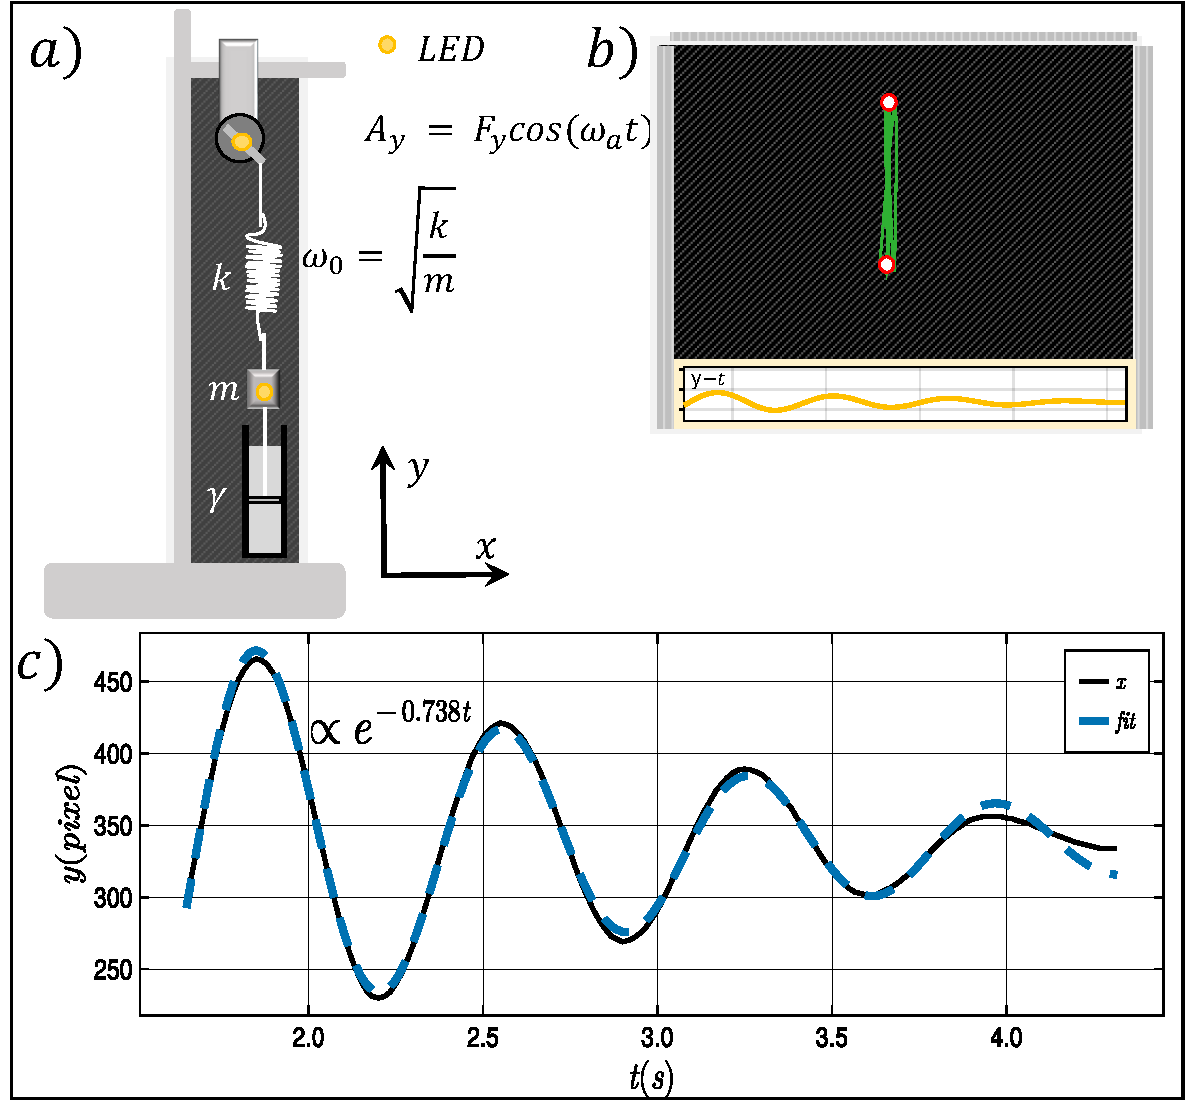
\includegraphics[width=12 cm]{figures/Damped Harmonic Motion.pdf}
    \caption{(a) The experimental setup of the driven harmonic oscillator. The periodic force $A_y$ stretches the spring, which results in a (counter) force $F_y = -ky$. The result is a resonance system with viscous damping $\gamma$. (b) The result of the object tracking using MaxTRAQ 2D. (c) A plot of the y-coordinate of the object as a function of time. Note that there is not external driving force $A_y=0$, so we have damped harmonic motion.}
    \label{Figure: DDHM}
\end{figure}

\subsubsection{Phase-space (hard)}    
Show that the phase-space plot x-v (or p = mv) consist of inward spiraling circles. The staring point of this project is to investigate a dynamical system:

\begin{align}
    x(t) = Ae^{-\zeta\omega_0t}\cos(\omega_1 t) & \\
    v(t) = -A \zeta \omega_0 e^{\zeta \omega_0 t} - A \omega_1e^{\zeta \omega_0 t}\sin(\omega_1 t).
\end{align}
If we plot the position against the velocity the phase-space plot shows a circle. What is the interpretation of the circle (Energy). Why is the circle inward spiraling and can we show the theoretical curve on top of the phase-space picture? To do this, the students have to calculate the frequency $\omega_0$ and the damping coefficient $c$. Then, you can make a theoretical prediction of x(t) and v(t) and compare these with the experimental results. This project can be seen as an extension of the previous experiment on simple damping.

\newpage

\subsection{Coefficient of restitution of a ball}
\subsubsection{Theory}
When e.g. a football falls down from a height $h$ the potential energy is converted into kinetic energy. The velocity at the ground can be calculated by an energy balance:
\begin{align}
    E_{pot} = E_{kin} & \\
    v = \sqrt{2gh}.
\end{align}
When the ball hits the ground, a part of the energy is transferred to the ground, hence the velocity after hitting the ground $v'$ is lower than the initial velocity $v'< v$. 

The ratio of the velocities is known as the coefficient of restitution:

\begin{equation}
    \epsilon = \frac{v'}{v} = \sqrt{\frac{h'}{h}}.
\end{equation}

with $\epsilon$ the coefficient of restitution and $h'$ the maximum height the ball reaches after the collision. Without any transfer of energy, i.e. a perfect elastic collision, the velocities $v'$ and $v$ are the same, hence $\epsilon = 1$. An (ideal) inelastic collision means that the final velocity $v'$ is zero, hence $\epsilon = 0$.

The coefficient of restitution depends on the material of the ball and, even more important, the pressure inside the ball. 

In the paper "\textit{Coefficient of restitution of pressurized balls: a mechanistic model}" the authors investigate the role of pressure and the corresponding coefficient of restitution.

They assume that the football consists of an elastic material $k$ that stores (potential) energy during the compression at the impact. Furthermore, they assume that there's a dissipative force $F_d$ during the compression and decompression. Using these assumptions they show that the energy balance during compression is given by:

\begin{align}
    E_c = \frac{1}{2}kx^2 - mgx +F_d x.
\end{align}

Likewise, during decompression the energy balance reads:

\begin{align}
    E_d = \epsilon^2 E_c= \frac{1}{2}kx^2 - mgx - F_d x,
\end{align}
with $\frac{1}{2}kx^2$ the potential energy stored by the (de)compression $-mgx$ the potential energy of the ball and $F_dx$ the dissipated energy. Furthermore, they assume that part of the energy $\epsilon^2$ is transferred during the (de)compression, $E_d = \epsilon^2E_c$.

The sum and difference of these equations read:

\begin{align}
   E_c(1+e^2) = kx^2 -2mgx &\\
   E_c(1-e^2) = 2F_dx,
\end{align}
the ratio of these equations is:

\begin{align}
    \frac{1+e^2}{(1-e^2)^2} = \frac{(kx^2 -mgx) E_c}{4F_dx^2} & \\
    \frac{1+e^2}{(1-e^2)^2}  \approx \frac{k E_c}{4F_d}.
\end{align}

The last line assumes that the stored energy is larger than the potential energy inside the ball $(1/2)kx^2>>mgx$. Next, they show that the spring constant $k$ is given by:

\begin{align}
    k = 2\pi R P_g + 4\pi GD_w,
\end{align}
with $G$ the shear modulus, $R$ the radius of the ball, $D_w$ a constant (?) and $P_g$ the gauge pressure inside the ball. The details are not so relevant, but qualitatively it shows that the restoring force $kx$ depends on the two factors. $2\pi R P_g x$ a 'Hookean' restoring force as a result of the compression of the ball and a restoring force that arises from the deformation of the wall $4\pi G D_w x$.

Combing the equations above we arrive to:

\begin{align}
    \frac{1+e^2}{(1-e^2)^2}  = A P_g + B,
\end{align}
with $A = \frac{\pi R E_i}{2F_d^2}$ and $B = \frac{\pi GD_wE_i}{F_d^2}$. Both A and B are constants and do not have a clear physical meaning.

The ratio ($(E_c+E_d)/(E_c-E_d)^2$) is linear in the ball pressure if the energy stored in the compression of the ball is much larger than the potential energy still available in the ball (this is not the potential energy at the start of the experiment. This is the potential energy that is still there during the compression, so almost zero.). This is true for most sports balls. It is
certainly true for any ball stiff enough to support its own weight
at zero gauge pressure without being significantly deformed.

\subsubsection{Setup and results}
In this experiment the students can study various elastic sport balls. An example setup is shown in Fig. \ref{Fig. falling object}. In this specific experiment a basketball was used. An LED was attached on top of the ball to track the position. The ball was released from a height $h$. The velocity at the ground can be calculated using $v = \sqrt{2gh}$. The ball was released carefully to minimize velocities in the x-direction.

If we assume that air-resistance is negligible the y-position of the basketball is given by:

\begin{align}
    y(t)-y_0 = (-)\frac{1}{2}gt^2,
\end{align}

with $g$ the gravitational acceleration. The parabolic motion is clearly visible in Fig. \ref{Fig. falling object} c. The coefficient of restitution can easily be extracted by calculating the ratio of consecutive heights:

\begin{align}
    \epsilon = \sqrt{\frac{h_{i+1}}{h_{i}}},
\end{align}
with $h_i$ the height at bounce $i$. A different approach is to calculate the time of flight (TOF) between each bounce. 

The TOF for a ball that starts with initial velocity $v_0$ (the velocity after the bounce) is given by:
\begin{align}
    t_{TOF} = \frac{2v_0}{g}.
\end{align}

The TOF ratio between two consecutive bounces is therefore:

\begin{align}
    \frac{t_{TOF,i+1}}{t_{TOF,i}} = \frac{v_{i+1}}{v_i} = \epsilon,
\end{align}
which is exactly the ratio of the velocities, hence the coefficient of restitution.

The y-position of the basketball is shown in Fig. \ref{Fig. falling object} c. The first (half) bounce is removed from the data. The data shows the maximum heigh of each of the bounces (y-axis) and the TOF during each bounce (x-axis).

\begin{figure}[H]
    \centering
    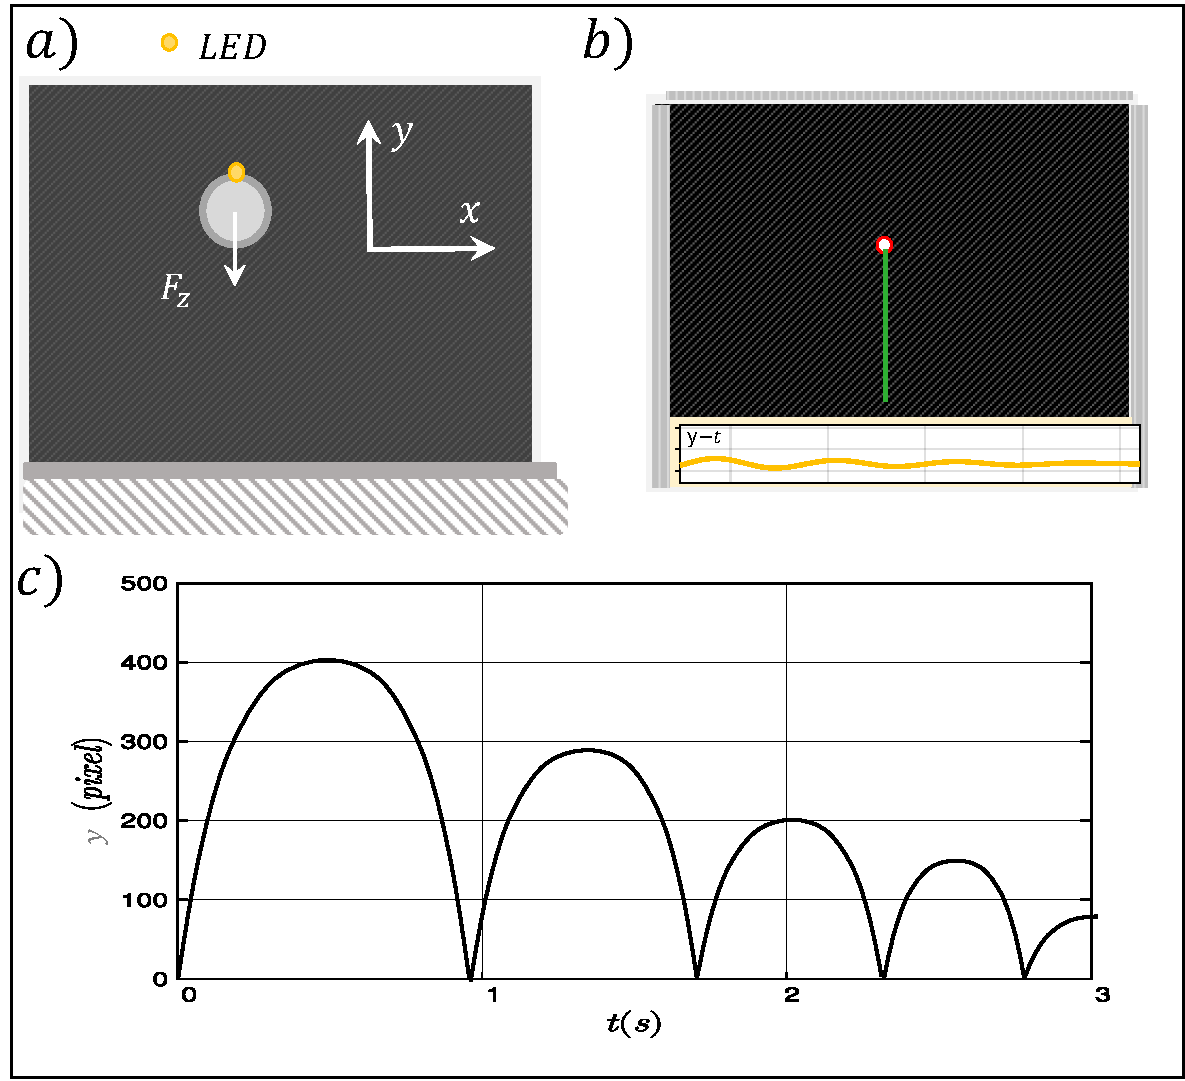
\includegraphics[width = 12cm]{figures/Falling_object.pdf}
    \caption{The falling basketball experiment. a) A schematic representation of the basketball. An LED was placed on top of the basketball. In b) the tracked position of the LED lights is shown. Obtained using MaxTRAQ 2D. c) The tracked y-position of the basketball. The first (half) bounce was removed from the data. The data shows 5 bounces.}
    \label{Fig. falling object}
\end{figure}

\subsubsection{Calculate the coefficient of restitution of a ball(very easy)}    
In this experiment the students can calculate the coefficient of restitution $\epsilon$ of various balls. The coefficient of 
restitution can be calculated with the following two formulas:

\begin{align}
    \epsilon = \sqrt{\frac{h_{i+1}}{h_{i}}},
\end{align}
with $h_i$ the height at bounce $i$ and 
\begin{align}
    \epsilon = \frac{t_{TOF,i+1}}{t_{TOF,i}} = \frac{v_{i+1}}{v_i},
\end{align}
with $t_{TOF,i}$ the time of flight for bounce $i$.

\subsubsection{Varying the pressure (hard)}    
Show that ratio $(E_c+E_d)/(E_c-E_d)^2$ is linear in the gauge pressure. Combing the equations above we arrive to:

\begin{align}
    \frac{1+e^2}{(1-e^2)^2}  = A P_g + B,
\end{align}
with $A = \frac{\pi R E_i}{2F_d^2}$ and $B = \frac{\pi GD_wE_i}{F_d^2}$. Both $A$ and $B$ are constants and do not have a clear physical meaning.

Students can use the literature review as inspiration and theoretical background. In the experiment it is best to use a basketball and increase the pressure of the ball. Otherwise the ball will deform too much and the theory does not apply anymore.

Lastly, the linear equation is not a simple equation $e$. By using some elementary algebra the students can find a function of $e$ versus the gauge pressure $Pg$. First we define $k = A P_g + b$ and $x=e^2$, hence:

\begin{align}
    \frac{1+x}{(1-x)^2} = k & \\
    (1+x) = x^2 k - 2xk +k & \\
    x^2 k - x(2k+1) + (k-1) = 0, & \\
\end{align}
next we apply the quadratic formula and solve for $e$:
\begin{align}
    x_{\pm}  = \frac{(2k + 1) \pm \sqrt{(2k+1)^2 - 4(k-1)k}}{2k} & \\
    x_{\pm}  = \frac{(2k+1) \pm \sqrt{4k^2 +4k + 1 -4k^2+4k}}{2k} & \\
    x_{\pm}  = \frac{(2k+1) \pm \sqrt{8k + 1}}{2k} & \\ 
    x_{-}  = 1+ \frac{1-\sqrt{8k + 1}}{2|k|}& \\ 
    e = \sqrt{1+ \frac{1-\sqrt{8(AP_g+B) + 1}}{2(AP_g+B)}}.
\end{align}
Note that it is useful for the students to derive this result themselves (they should be able to do this). The TA should guide them through this process and alert the students to pick only one of the solutions of the quadratic equations. They should argue that you can only pick $x_{-}$, otherwise the coefficient of restitution can exceed 1.
\newpage


\subsection{Rotating Wheel}
This section is originally developed by T.W. Hijmans.
\subsubsection{Theory}
In this experiment, we examine a transparent plexiglass hollow wheel containing a viscous fluid. This problem finds its application in cycling. Mountain bikes, as well as road bikes increasingly, use tubeless tires. These tires are devoid of inner tubes and provide an airtight seal with the rim, containing a latex-based fluid. These tires are lighter than ones with inner tubes, and the vulcanizing fluid automatically seals small leaks. In this experiment, we investigate the influence of the internally present fluid on the rolling resistance of such a wheel.

\begin{figure}[H]
    \centering
    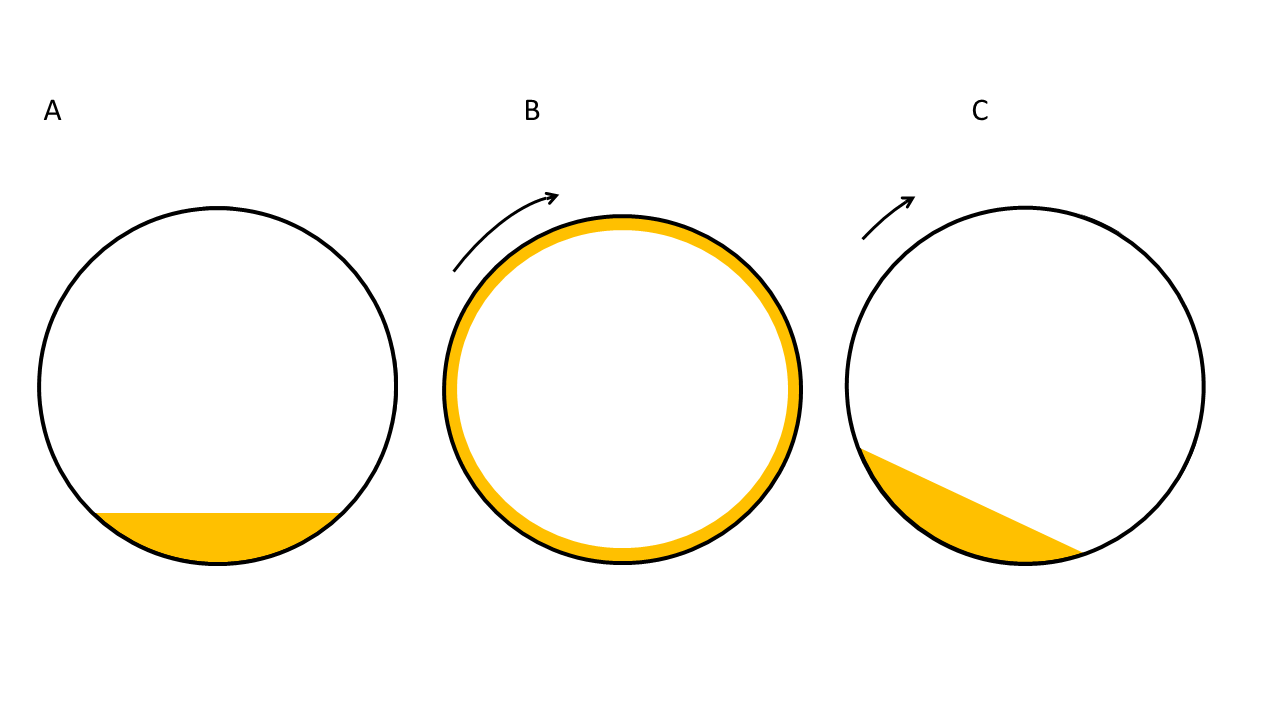
\includegraphics[scale=0.35]{figures/wiel.png}
    \caption{A hollow wheel filled with fluid. In situation A, the wheel is not rotating, and the fluid collects at the bottom. In situation B, the wheel rotates rapidly, causing the fluid to spread as a film across the entire inner wall due to centrifugal force. In situation C, the wheel rotates slowly. In this case, the slightly off-center puddle of fluid induces a frictional force that slows down the rotation of the wheel.}
    \label{Fig. wheel}
\end{figure}

We will replace the "tire" mentioned in the introduction with a hollow plastic wheel filled with fluid made of transparent plastic (see Fig. \ref{Fig. wheel}). Let's first consider three situations: A) a stationary wheel with the fluid collecting at the bottom, B) a wheel rotating at high speed, where the fluid forms a film on the inner side due to centrifugal force, and finally, C) a situation where the wheel rotates slowly, causing the fluid to move but not fully coat the entire inner side. In situation B (high rotational speed), we expect the fluid film to move along with the rotating wheel. The only difference from a wheel without fluid is that the mass and moment of inertia of the wheel slightly increase due to the presence of the fluid film. The angular frequency at which the wheel rotates will decrease over time due to air resistance and friction in the wheel bearings, but these forces are practically small.

In situation C, the rotational speed is so low that the fluid remains at the bottom of the wheel under the influence of gravity. Due to the friction between the fluid and the wheel, we can expect the fluid to be partially dragged along by the wheel, creating a situation similar to panel C in Fig. \ref{Fig. wheel}. Two forces act on the fluid, balancing each other: gravity, which tries to bring the puddle of fluid to the lowest point of the wheel, and the frictional force with the wall that drags the fluid. Thus, the equilibrium position of the fluid is determined by the rotational speed of the wheel.

The rotational speed $v_o$ that determines the transition between regimes B and C in Fig. \ref{Fig. wheel} is given by:
\begin{equation}
    \frac{v_o^2}{R} = g, \label{eq:centrifuge}
\end{equation}
where $R$ is the radius of the wheel, and $g$ is the acceleration due to gravity. The speed $v_0$ is related to the angular velocity $\omega$ of the wheel by:
\begin{equation}
    v_o = \omega R. \label{eq:v0=omegaR}
\end{equation}

There are various possibilities for the resistance force that slows down the wheel. First, let's consider the situation without fluid in the wheel. If there is a "classical" frictional force, i.e., a force (or more accurately, an angular acceleration) that is independent of the rotational speed, we have:
\begin{equation}
    \frac{\mathrm{d} \omega}{\mathrm{d} t} = - \lambda_0, 
    \label{lambda0}
\end{equation}
where $\lambda_0$ is a constant.
Alternatively, we can assume that the frictional resistance experienced by the empty wheel is proportional to the angular velocity:
\begin{equation}
    \frac{\mathrm{d} \omega}{\mathrm{d} t} = - \lambda_1 \omega, \label{lambda1}
\end{equation}
where $\lambda_1$ is a new constant describing this case.
Lastly, we can assume that air resistance is the main factor, in which case we have:
\begin{equation}
    \frac{\mathrm{d} \omega}{\mathrm{d} t} = - \lambda_2 \omega^2, 
    \label{lambda2}
\end{equation}
where $\lambda_2$ is a constant. It is possible that multiple types of resistance forces are simultaneously active.

When we fill the wheel with fluid and rotate it rapidly (situation B in Fig. \ref{Fig. wheel}), the angular acceleration is given by equations (\ref{lambda0}) to (\ref{lambda2}), but with slightly different values for the constants $\lambda_0$, $\lambda_1$, and $\lambda_2$ due to the increased mass and moment of inertia.

The last, and most interesting for us, case is $v < v_0$, corresponding to panel C in Fig. \ref{Fig. wheel}. Without proof, we mention that in this case, we can expect the frictional force to be quadratic in velocity. In this case, equation (\ref{lambda2}) applies again, but now with a much larger value of $\lambda_2$ due to the stronger interaction between the wheel and the viscous fluid.

\subsubsection{Setup and results}
In this experiment the student will use a rotating wheel. A schematic setup is shown in Fig. \ref{Fig. Rotating Wheel}a). The positioning of the LED lights is essential and one LED needs to be attached to the outer surface, to maximize contrast we place the setup behind a black cardboard sheet. The second LED can be positioned in the center of the wheel. Obtaining a clear footage is difficult and it is worth to invest the time in optimizing the camera position. During the analysis the LED light can move behind the wheel pole, this is inevitable and it is still feasible to do the tracking. In Fig. \ref{Fig. Rotating Wheel} b) we show the tracked path of the LED lights. In Fig. \ref{Fig. Rotating Wheel} c) the x-position of the tracked position is shown, a peek-finding algorithm was used to detect the maxima and minima.

The x-position (or y-position) of the LED light shows a dissipating oscillating signal. However, the type of dissipation is unknown in this case. That means that we do not have a closed-form analytical solution for the x-position as a function of time. To calculate the angular velocity $\omega$ we have to calculate it at different time intervals. The procedure is as follows: find the time interval $T_{a-b}=T_a-T_b$ between the neighboring maxima (or minima). Convert this to an angular frequency by $\omega_{a-b} = \frac{2\pi}{T_{a-b}}$ and denote the center time $t_{a-b}$ between $T_a$ and $T_b$. This procedure should be done with all the minima and maxima. The procedure is tedious and labour intensive (you can use a programming language to speed this up), but the result is a graph of $\omega$-t. The time derivative can also be visualized $\frac{d\omega}{dt}-t$ and should be compared to the theoretical prediction. An example analysis of a empty wheel is shown in Fig. \ref{Fig. Rotating Wheel} e).

\begin{figure}
    \centering
    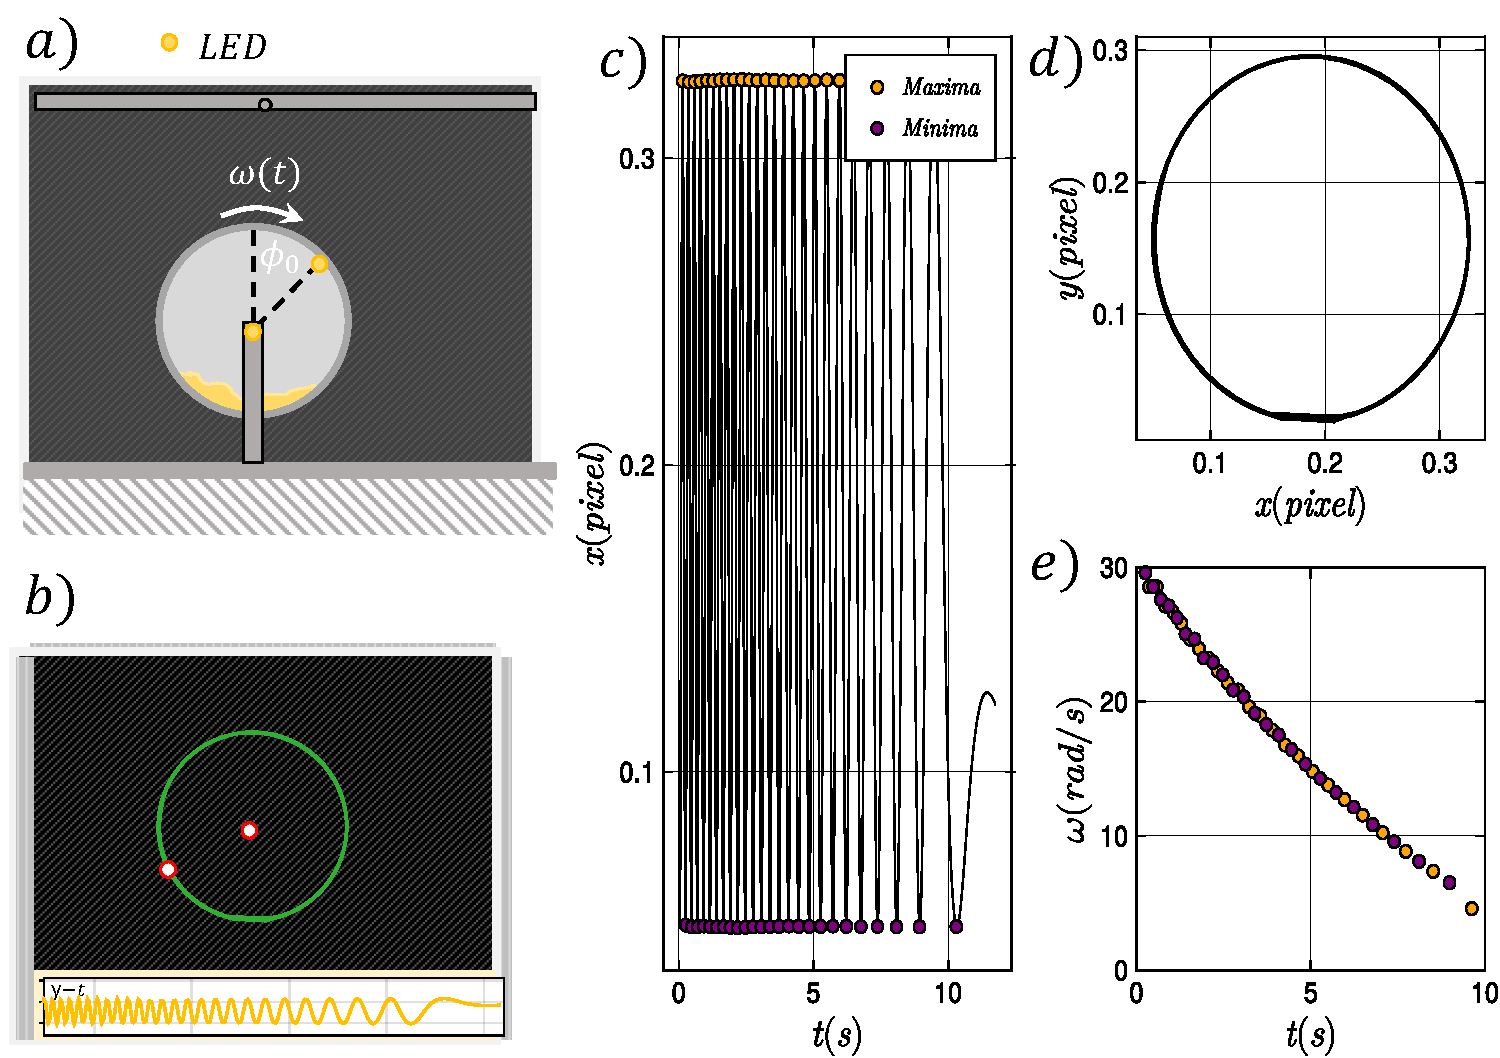
\includegraphics[width=12cm]{figures/Rotating Wheel.pdf}
    \caption{The rotating wheel experiment. a) The schematic setup of the rotating wheel experiment. The wheel is rotating at an angular velocity $\omega$, but it experiences an unknown frictional force that slows the rotational motion down. The LED light capture the slowing down of the angular frequency. In b) the the tracked position is shown using MaxTRAQ 2D. In c) the tracked x-position is shown and in d) the x-y plane is shown. In c) the yellow and purple dots correspond to the maxima and minima of the position. They were found using a peak finding algorithm. Using the difference between each of the maxima the angular frequency is calculated. It is clear that the angular frequency experiences a friction forces.}
    \label{Fig. Rotating Wheel}
\end{figure}

\subsubsection{Friction of a empty rotating wheel (hard)}
Try to analyze the camera footage to observe how the angular velocity of the wheel changes due to the frictional effect. Start the experiment by examining a wheel without fluid. Pay close attention to visually observe what happens around this transition point.

By analyzing the camera footage, you can track the changes in angular velocity as the wheel rotates. It is important to visually observe the wheel's behavior to gain a comprehensive understanding of the dynamics involved.

Try to find how the angular frequency changes in time. The frictional forces that are dominant depend on the angular velocity as well, try to maximize the angular velocity and observe the behavior. 

\subsubsection{Friction of an oil filled rotating wheel (hard)}
Try to analyze the camera footage to observe how the angular velocity of the wheel changes due to the different friction effects. It would be helpful to start by examining a wheel without fluid. When observing the filled wheel, we expect that when we start with a rapidly rotating wheel, at a certain point (i.e., when the velocity drops below the critical threshold of Eq. \ref{eq:v0=omegaR}), a new regime with significantly increased friction will be reached. Pay close attention to visually observe what happens around this transition point.

By analyzing the camera footage, you can track the changes in angular velocity as the wheel rotates. Look for any distinct patterns or behaviors that occur during the transition from one regime to another. It is important to visually observe the wheel's behavior to gain a comprehensive understanding of the dynamics involved.



\newpage

\subsection{Rolling Cylinder}
\subsubsection{Theory}
In this experiment the students will roll down an object from an incline. The initial energy of the system $E_i$ is potential energy that depends on height (difference) $E_i = mgh$. When the object starts rolling down the incline the potential energy is converted to kinetic energy and rotation energy. The rotational moment of the object depends on the moment of inertia of the object. The moment of inertia of standard geometric object is well know and has the form $I = bmr^2$, with m the mass of the object, r the radius of the object and b a geometric dependend constant. Next, we assume that the kinetic energy of the object is the result of the rotational motion of the mass i.e. $v = \omega r$ and not an extra sliding velocity we can write the energy balance as
\begin{align}
    E_i = E_f & \\
    mgh = \frac{1}{2}mv^2 + \frac{1}{2}I\omega^2. & \\
\end{align}
Next, we solve for the velocity and we find 

\begin{align}
    v = \sqrt{\frac{gh}{1+b}}.
\end{align}
If we are interested in the acceleration we have to differentiate the velocity with respect to the time, i.e. 

\begin{align}
    \frac{d}{dt}(v^2) =\frac{d}{dt} (\frac{gh}{1+b}) &\\
    2v\dot{v} = \frac{g\dot{h}}{1+b} & \\
    a = \frac{g\sin(\theta)}{1+b},
\end{align}
where I used the chain-rule in the first line and used that the velocity along the incline $v$ is related to the vertical velocity $\dot{h}$ by $\dot{h} = |v|\sin{\theta}$. If we assume that the initial velocity is zero $v(0) = 0$ and that object starts at position $x_0$ can solve for the x-position as a function of time:

\begin{align}
    x(t) - x_0 = at = \frac{g\sin(\theta)}{1+b}.
    \label{eq: rolling cylinder}
\end{align}
The moment of inertia of geometric objects can be found in any classical mechanics textbook, for a sphere we have $=\frac{2}{5}mr^2$,so $b=\frac{2}{5}$. Thus the acceleration of a sphere along an incline is $a = \frac{5}{7}g\sin(\theta)$. If we look at the ratio between the acceleration and gravitation force on the incline, we have $a/(g\sin(\theta) = \frac{5}{7}<1$ the reduced acceleration is slower as a result of the inertial moment of the object. Similarly, the reduced acceleration of a cylinder $a / g\sin(\theta) = 2/3$ is smaller than the reduced acceleration of a sphere, this is the result of a different distribution of mass. The "centre of mass" of half a cylinder is more outward distributed compared to the sphere, the resulting acceleration is therefore lower.

\subsubsection{Setup and results}
In this experiment the students can use multiple objects with varying moment of inertia to investigate the moment of inertia. An example setup is shown in Fig. \ref{Fig. rolling cylinder}. In this case an LED was attached to the side of a (hollow) cylinder. Ideally, one would attach the LED light to the center of the cylinder. Due to practical matters it is sometimes very difficult to attach the LED in the centre, hence the LED was placed at a distance $\gamma r$ of the cylinder, with r the radius of the cylinder and b is the fraction of the radius where the LED is attached (b = 0 if the LED is placed at the centre of the cylinder, b = 1 at the edge of the cylinder). 

When the cylinder starts rolling, the tracked LED will experience an additional rotating motion $r_{rot}$, see Fig. \ref{Fig. rolling cylinder} b. The x-position of the rotating motion of the LED can be expressed as:

\begin{equation}
    x_{rot} = br\cos(\omega t + \phi),
\end{equation}
with $\omega = \frac{v}{r}$ the rotation motion of the LED. Since the velocity increases linear, we can express the rotational velocity as $\omega(t) = \frac{a t^2}{r}$. By combining these result with the previous result of the x-position we arrive to the equation of the x-position as a function of time:

\begin{align}
    x(t) - x_0 = at +x_{rot}(t) & \\
    x(t) - x_0 =  \frac{g\sin(\theta)}{1+b}t + \gamma r\cos(\frac{
        g\sin(\theta)t^2}{(1+b)r} +\phi).
    \label{eq: rotational motion cylinder}
\end{align}
An example trajectory (+ fit) is shown in Fig. \ref{Fig. rolling cylinder} c/d.

\subsubsection{Gravitational acceleration (both easy and hard)}    
Calculate the gravitational acceleration $a$ using different angles $\theta$:

\begin{align}
    x(t) - x_0 =  \frac{g\sin(\theta)}{1+b}
\end{align}
In this experiment the students can calculate the gravitational acceleration of a rolling object. The students can choose between various objects e.g. (metal) spheres, (hollow) cylinders, etc. The moment of Inertia of these objects is known and students should look this up (or calculate if necessary). \\

By varying the angle $\theta$ the students can observe a change in the acceleration $a$ of the object. By studying multiple angles the students can make a graph of the acceleration versus the (sine) of the angle $\theta$. The slope of the graph is $g/(1+b)$, the students can verify this. Similarly, by assuming that $g = 9.81$ students can check if $b$ is the correct value for their shape. \\

A more complicated approach is to attach the LED at a distance $\gamma r$ of the cylinder. The research questions are the same, but the analysis is much more complicated. During the analysis the students should fit Eq. \ref{eq: rotational motion cylinder}, this is difficult. A good starting approach is (as always) to measure $r$, $\gamma$ and start with a simple quadratic equation. When the quadratic fit works (excluding the oscillating part), add the rotational part.





\begin{figure}
    \center
    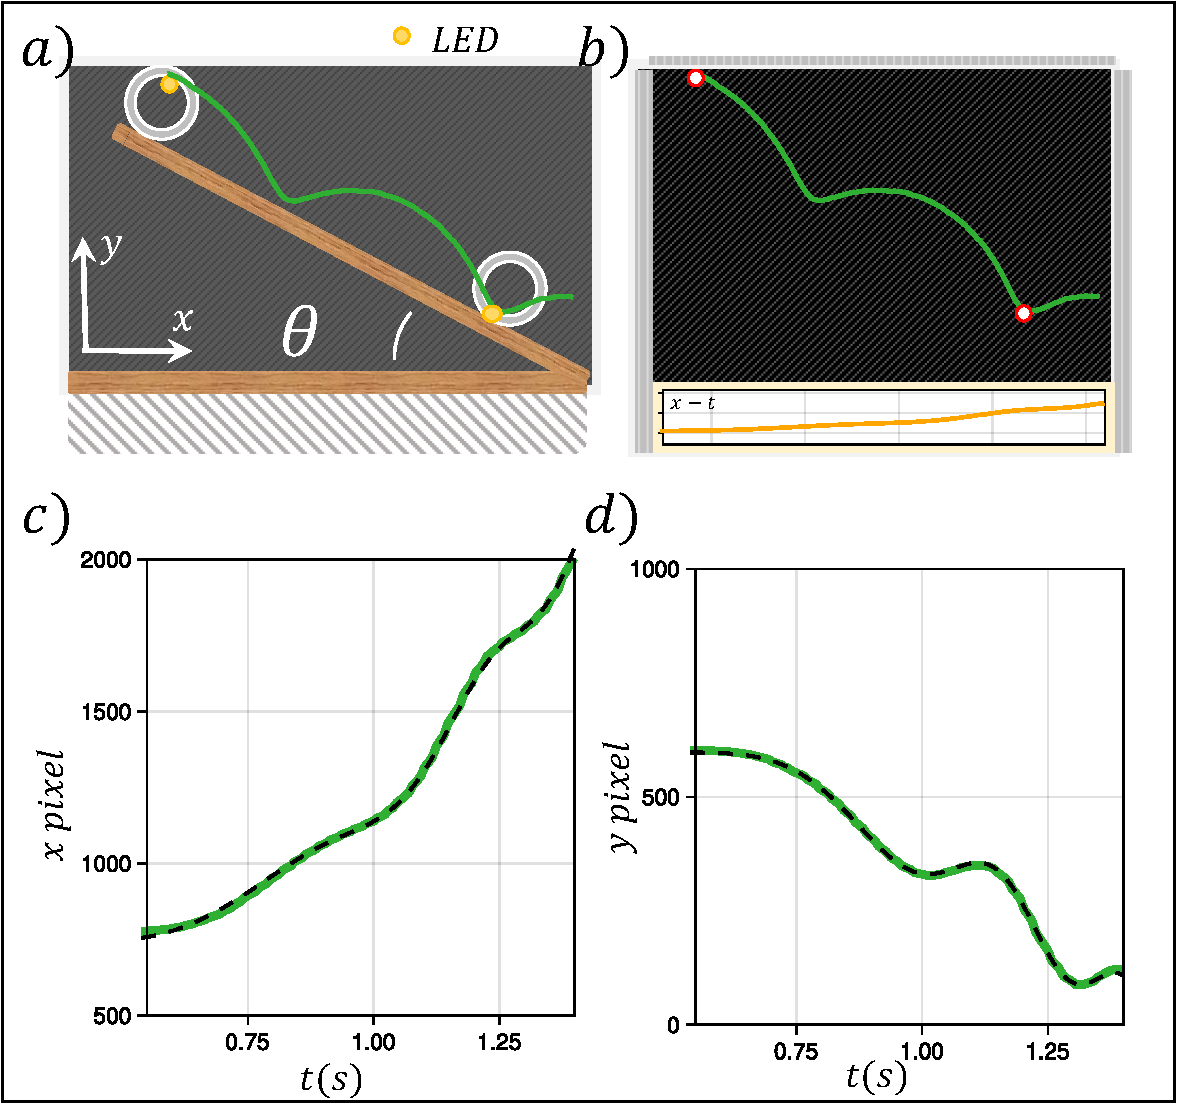
\includegraphics[width = 12 cm]{figures/Rolling Cylinder.pdf}
    \caption{The moment of inertia experiment. a) The schematic setup of the rolling cylinder. The cylinder rolls down the incline with acceleration a. The acceleration depends on the mass distribution, hence the shape of the object. In this case the LED was attached to a hollow cylinder at position $\gamma r$. In b) the tracked position is shown using MaxTRAQ 2D. In c/d the x/y position of the LED is shown. The x/y-position experiences a constant gravitational force, hence it shows a quadratic shape. On top of the quadratic shape the LED experiences a rotational motion $x/y_{rot}$. Eq. \ref{eq: rotational motion cylinder} was used to fit the data. The fit provides information of the following parameters: $a$, $x_0$, $\gamma$ and $\phi$.}
    \label{Fig. rolling cylinder}
\end{figure}
\newpage

\subsection{Chaotic pendulum}
\subsubsection{Theory}
A chaotic system is a mathematical model that exhibits sensitive dependence on initial conditions, a property known as "chaotic behavior." Such systems are typically described by nonlinear equations and demonstrate complex, intricate, and seemingly random patterns in their dynamics. 

One defining characteristic of chaotic systems is their sensitivity to initial conditions, often referred to as the "butterfly effect." Even small changes in the starting state of a chaotic system can lead to dramatically different trajectories and outcomes. This sensitivity arises from the amplification of initial perturbations through the nonlinear interactions within the system, ultimately resulting in diverging behaviors.

Despite being deterministic, chaotic systems display behavior that appears random and unpredictable over long time scales. This unpredictability arises from the exponential divergence of trajectories in phase space, rendering long-term predictions highly challenging.

There are a few conditions that defines a chaotic system:
\begin{itemize}
    \item Sensitive to initial conditions;
    \item Dense periodic orbits;
    \item Topological transitive.
\end{itemize}
The first condition is referred to as the "Butterfly effect". The second condition is less trivial. A linear system has a single predictive orbit (in for example phase space) that is constant, a chaotic system however can have a very dense orbit structure. By changing for example, the driving amplitude of a mathematical pendulum we can have a cascade structure of orbits (a period double sequence). The last condition, topological transitivity, refers to a property of dynamical systems where the trajectories or paths of the system can visit every part of its phase space. In simpler terms, it means that no matter where you start within the system, you can eventually reach any desired location.

The second and third conditions are very hard to observe in an experimental system and a way beyond the level of a second year student. The first condition however, is relatively easy and can be characterized by a Lyapunov exponent.

Given two starting trajectories in the phase-space with initial separation $\delta d_0| = |d_1-d_2|$, the separation grows exponentially according to

\begin{align}
    |\delta(t)|\approx |\delta d_0|e^{\lambda t}.
    \label{Eq. Lyapunov}
\end{align}

$\lambda$ is referred to as the Lyapunov exponent. If $\lambda < 0 $ the trajectories converge and the orbit is exponentially stable. If $\lambda = 0$ the trajectories do not converge, nor will they diverge, they are stable. Stability does not imply that their distance stays constant, but that they are not attracted to a stable manifold.

The last scenario, $\lambda>0$, implies instability. The nature of the chaotic system results in diverging trajectories. This is independent of the initial separation.

For a linear pendulum we can derive the Lyapunov exponent by hand. We start by defining two trajectories $\theta(t)$ and $\theta'(t)$ that are separated by a small difference in their phase $\epsilon$. The time-evolution of $\theta$ is given by the linear oscillator equation
\begin{align}
    \theta(t) =A\cos(\omega t + \phi),
\end{align}
with A the amplitude, $\omega$ the eigenfrequency of the pendulum and $\phi$ the starting angle. The separation between the oribits is now given by:
\begin{align}
    |\delta \theta(t)| = \theta(t)-\theta'(t) & \\
    = A\cos(\omega t + \phi) - A\cos(\omega t +\phi +\epsilon) & \\
    = A\cos(\omega t + \phi) - A\cos(\omega t +\phi)\cos(\epsilon) +A\sin(\omega t +\phi)\sin(\epsilon) & \\
    \approx A\cos(\omega t + \phi) - A\cos(\omega t +\phi) +A\sin(\omega t +\phi)\epsilon & \\
    \approx  |\epsilon A \sin(\omega t + \phi)|,
\end{align}
where I used that $\epsilon \ll 1 $ and Taylor expanded the cosine and sine up to first order $\cos(\epsilon)\approx1$ and $\sin(\epsilon)\approx\epsilon$. Furthermore I used the sum and difference formule of the cosine function. The separation $|\delta\theta(t)|$ follows a sine function with amplitude $A\epsilon$, hence the separation is not constant, but periodic in nature. However, the separation may not be constant, but the orbits do not diverge. This implies that the Lyapunov exponent is zero $\lambda =0$. 

\subsubsection{Setup and results}
In this experiment the students will use a pre-build double pendulum. A schematic setup is shown in Fig. \ref{Fig. Lyapunov}a). The LED lights should be attached at the end of each of the pendulum. To maximize contrast the experiment was placed behind a black cardboard sheet. During the analysis the LED light can move behind the first pendulum, this is should be avoided. In Fig. \ref{Fig. Lyapunov} b) we show the tracked path of the LED lights. In Fig. \ref{Fig. Lyapunov} c) the separation of the trajectories is shown, the black line is a fit using Eq. \ref{Eq. Lyapunov} with $\lambda>0$. 


\begin{figure}[H]
    \centering
    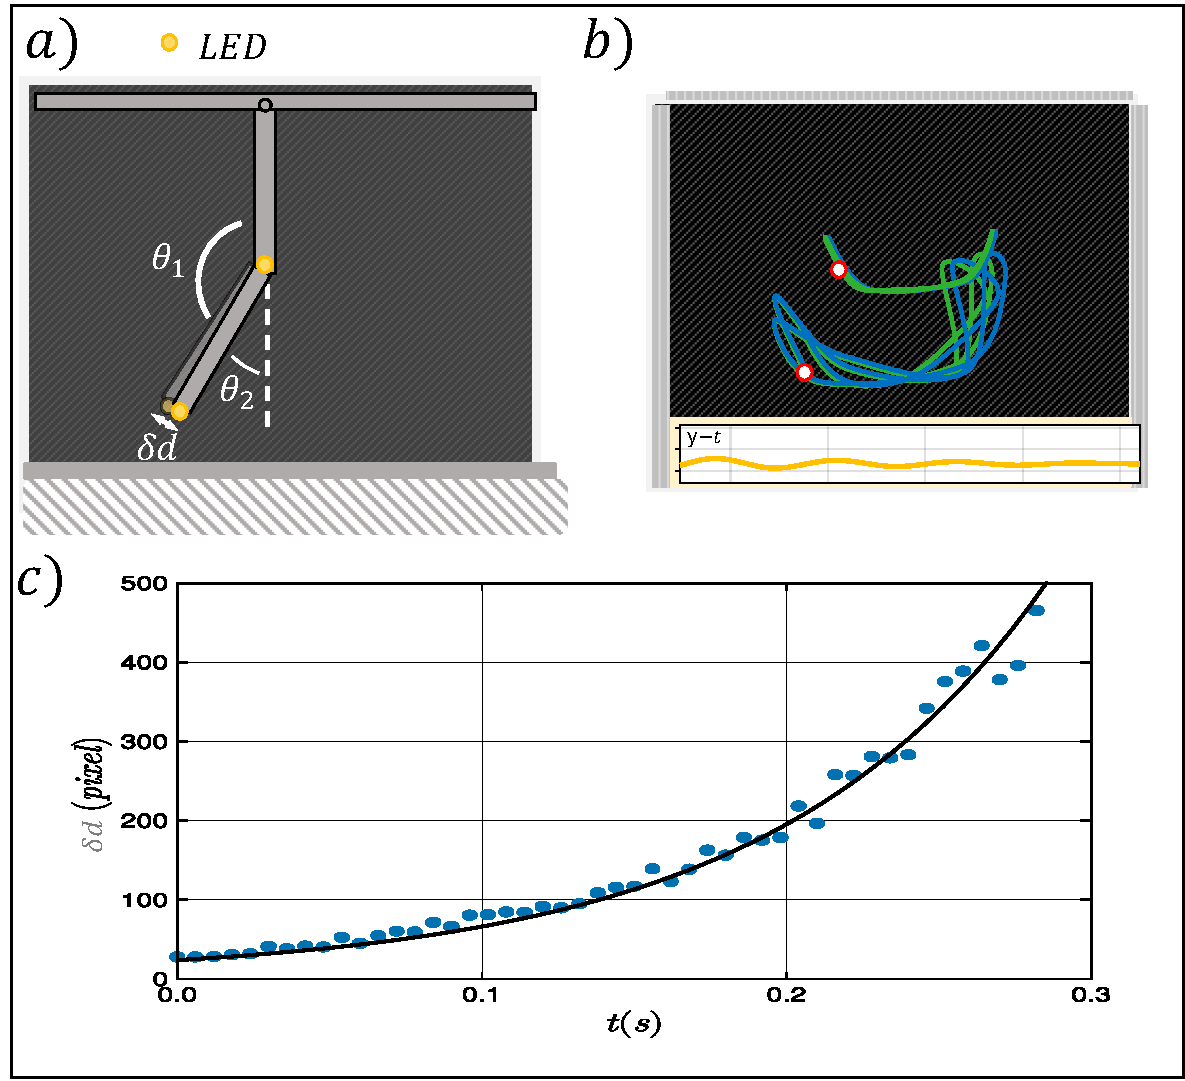
\includegraphics[width = 12cm]{figures/Lyapunov.pdf}
    \caption{The double pendulum experiment. a) A schematic representation of the double pendulum. The initial separation $\delta d$ is determined visually and must be minimized. The LED lights track the position of both pendula, this enables to construct a displacement vector of the second pendulum. In b) the tracked position of the LED lights is shown. The experiment is repeated twice, the individual trajectories are shown in blue and green. Obtained using MaxTRAQ 2D. c) The separation between the two trajectories shown in the first 0.3 seconds. The black line is a fit using Eq. \ref{Eq. Lyapunov}, with $\lambda > 0$. }
    \label{Fig. Lyapunov}
\end{figure}

\subsubsection{Lyapunov exponent (easy \& hard)}
The students can track the motion of the double pendulum by using small LED attached to the end of the pendulum. By tracking the motion of two similar release positions, the students can show that the system is chaotic.

The students can choose which parameter they want to track. For example, they can calculate the spatial difference between the two oscillators $\delta d = \sqrt{(x_1-x_2)^2+(y_1-y_2)^2}$, or, even better, they can track the difference in angle $\delta \theta = \theta_1-\theta_2$ between the two oscillators. The difference in angle $\theta$ is not bounded between $0$ and $2\pi$. In the book "Classical Mechanics" by Taylor, a very nice introduction to chaos theory is given. Students can use this book as a good reference and they can repeat some of the experiments.
\newpage

\subsection{Buoyancy}
\subsubsection{Theory}
Consider an experiment where a ball with density $\rho_b$ is immersed in a water tank containing water with a density of $\rho_w$. If the ball's density is less than that of the water ($\rho_b<\rho_w$), it will experience an upward force. The same reasoning also applies When the ball's density is larger than the density of water, then the ball will experience a downward force. The resulting force is known as the Buoyance force $F_b$. The concept of buoyancy force was first introduced by the ancient Greek mathematician and physicist Archimedes around 212 BC. This fundamental principle is now commonly referred to as Archimedes' Law.

In simple terms, the principle states that the buoyant force $F_b$
on an object is equal to the weight of the fluid displaced by the object, or the density $\rho$ of the fluid multiplied by the submerged volume V times the gravitational acceleration g.

We can express this relation in the equation:
\begin{equation}
    F_b = \rho_w V g.
\end{equation}
An object that floats on the surface has an buoyancy force that is equal to the weight of the object $F_g$. When the object is submerged we have the following situation:

\begin{align}
    ma = F_b - Fz & \\
    \rho_b V a = \rho_w g -\rho_b g & \\
    a = g(\rho_g/\rho_b - 1),
\end{align}
for $\rho_g/\rho_b < (>) 1$ the ball will sink (rise), since $a<(>) 1$. Next, we solve for $x(t)$ and assuming that $v(0)=0$:

\begin{align}
    x(t)-x_0 = \frac{g}{2} \left( \rho_g/\rho_b - 1 \right)t^2.
\end{align}

The ball will move quadratic with time, the only difference with Newtons falling apple, i.e. normal gravity, is the direction and the magnitude of the acceleration. If we know the density of the ball $\rho_b$ we can examine the physical properties of the fluid.

\begin{figure}[H]
    \centering
    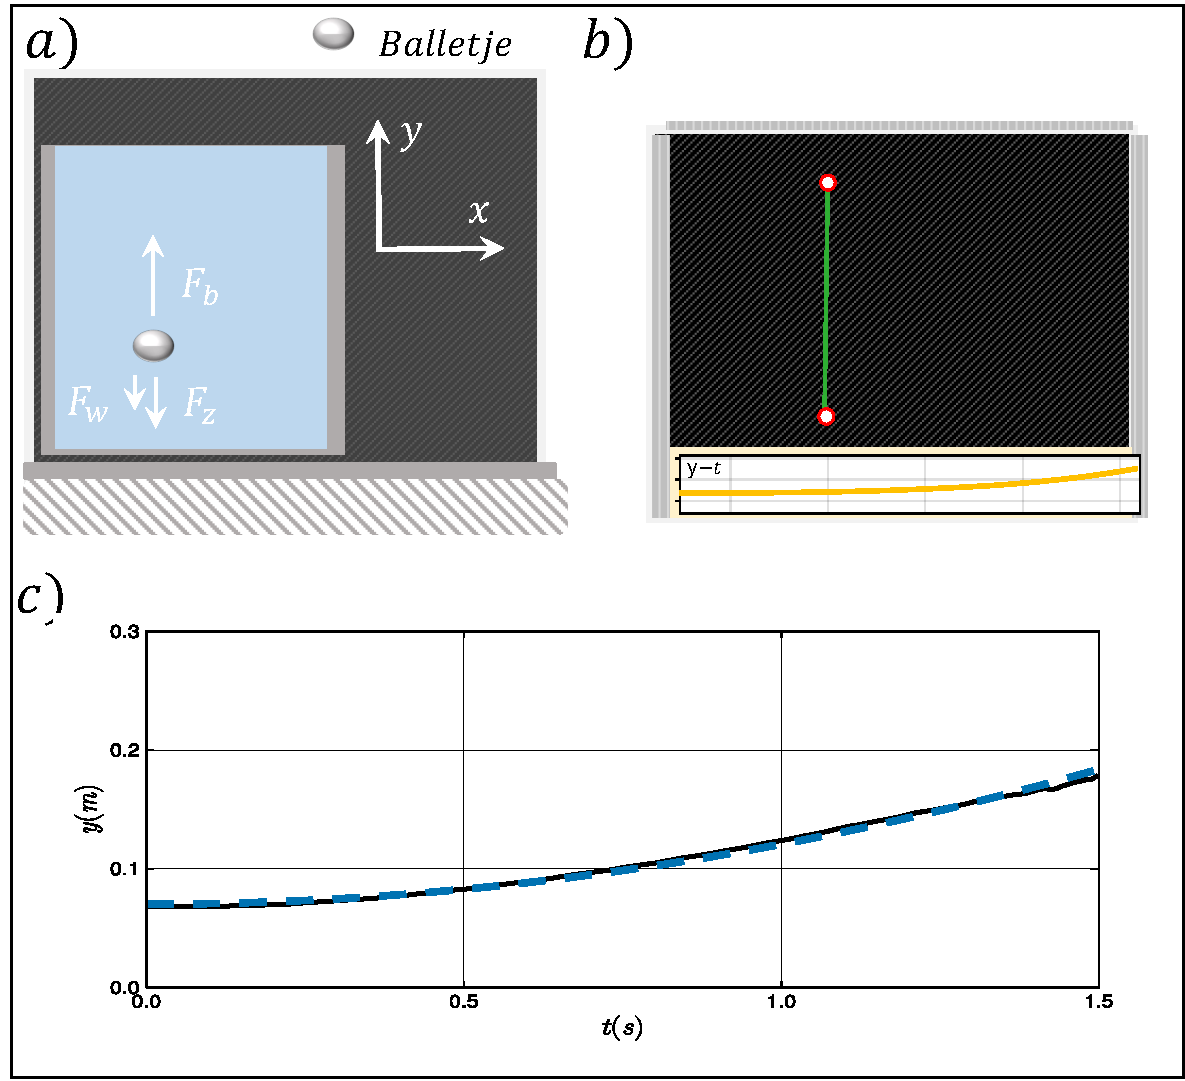
\includegraphics[width=12cm]{figures/Buoyancy.pdf}
    \caption{The setup of the buoyancy experiment. A ball of density $\rho_b$ is submerged into the water tank. The density of the ball and the water should be similar. The Lumenera Li255C captures the motion of the (rising) ball. The y-position of the ball is tracked using MaxTRAQ, the resulting movement is shown in the bottom of the graph.}
    \label{Figure: buoyancy setup}
\end{figure}

\subsubsection{Setup and results}
In this experiment the students can use a water tank (aquarium) to conduct their experiment. They should place a camera close the aquarium wall and maximize the contrast by using a (small) white ball. Furthermore, they should wear, preferably, black gloves and release the ball very careful. A slight instability at the moment of release of the ball will result in a drifting (out of plane) motion that is hard to track.
Lastly, the density of the ball should not differ to much from the density of water, otherwise the ball becomes untrackable. Students can alter the density of a regular ping-pong ball to control the density, and thereby the acceleration.

A schematic setup is shown in Fig. \ref{Figure: buoyancy setup}a. The tracked motion is shown in Fig. \ref{Figure: buoyancy setup}b.

\subsubsection{density of fluid (easy)}
In this experiment, students can determine the density of the fluid (or the ball) by analyzing the motion of the ball.

The acceleration of the ball is related to the density of the fluid ($\rho_f$) and the density of the ball ($\rho_b$) according to the formula:

\begin{align}
a = g \left(\frac{\rho_f}{\rho_b} - 1\right),
\end{align}

where $g$ represents the acceleration due to gravity, which is a known constant.

To determine the density of the fluid or the ball, students can analyze the motion of the ball and plot a graph of the vertical position (y) against time (t). The slope of this graph corresponds to the acceleration ($a$). By substituting the known value of $g$ and the measured acceleration ($a$) into the equation, they can solve for the density of the fluid or the ball, depending on which value they are interested in.

\subsubsection{friction of the ball (hard)}
In this experiment, students can explore the frictional behaviour of the ball in the fluid.

The experimental setup is equivalent to the previous proposed research question. However, in this case the students can analyze the data in more detail. Due to the frictional interaction between the surface and the fluid, the maximum velocity of the ball is capped. An extended force balance is needed:

\begin{align}
    ma = F_b - Fz - F_w,& \\
\end{align}
with $F_w$ the frictional force. If we assume that $F_w$ scales quadratic with the velocity (i.e. quadratic drag) $F_w = \frac{1}{2}C_w A \rho_w v^2$ we arrive to the following differential equation:

\begin{align}
    \rho_b V_b \ddot{x} = g\left(\rho_f-\rho_b\right)V_b -\frac{C_w A \rho_w}{2m} \dot{x}^2 & \\
    \ddot{x} = g \left(\frac{\rho_f}{\rho_b} - 1\right) - \frac{4C_w \pi r^2 \rho_w}{2m\rho_b \frac{4\pi r^3}{3}} \dot{x}^2 & \\
    \ddot{x} = g \left(\frac{\rho_f}{\rho_b} - 1\right) - \frac{3C_w \rho_w}{2m\rho_b r} \dot{x}^2,
\end{align}
where $r$ is the radius of the ball and I used that the ratio of the surface area to the volume of a sphere is $3/r$, $A/V = 3/r$. The solution can be found using elementary calculus (it looks more difficult than it actually is), although I would recommend to use WolframAlpha:

\begin{align}
    x(t) - x_0 = \frac{\log{(\cosh{(\sqrt{AB}t})})}{B},
\end{align}
with $A = g\left(\frac{\rho_f}{\rho_b}-1\right)$ and $B = \frac{3C_w A \rho_w}{2r\rho_b r}$. 
Lastly, the students can derive the terminal velocity $v_{\infty}$ by assuming that $ma = 0$, hence:

\begin{align}
    v_{\infty} = \sqrt{\frac{2rmg\left(\rho_f-\rho_b\right)}{3C_wA\rho_f}}.
\end{align}




\newpage

\subsection{Elastic Collisions}
\subsubsection{Theory}
Newton's Cradle is an iconic physics toy model that visualizes the principles of momentum and energy conservation. This simple device consists of a row of identical metal spheres suspended from a sturdy frame. When set in motion, it showcases a fascinating display of energy transfer and harmonic motion.

As each sphere swings back and forth, it collides with its neighboring sphere, during each collision the energy and momentum is transferred to the neighbouring sphere. Each collision is almost elastic, meaning that energy transfer is very efficient, hence the cradle will show many collisions before the energy is dissipated.

When the first ball $i$ with mass $m$ is released at height $h$, the system has a total kinetic energy of:

\begin{equation}
    E_i = mgh,
\end{equation}
with $m$ the mass, $g$ the gravitational acceleration and $h$ the release height. Just before the impact, the energy is full converted to kinetic energy by

\begin{align}
    v = \sqrt{2gh}.
\end{align}

During the impact a fraction of the energy is transferred to the neighbouring sphere $E_{i+1} = \epsilon E_i$, with $E_{i+1}$ the energy of the neighbouring ball. $\epsilon$ is the coefficient of restitution for the elastic collision, with $\epsilon<1$. After $n$ collisions the sphere will hit the final ball with energy 

\begin{equation}
    E_n = \epsilon^n E_i.
\end{equation}

The final ball will convert the kinetic energy to potential energy hence

\begin{equation}
    h' = \epsilon^n h.
\end{equation}
$h'$ is the maximum height of final ball. The coefficient of restitution is derived by

\begin{align}
    \epsilon = \left(\frac{h'}{h}\right)^{\frac{1}{n}}  = \sqrt[n]{\frac{h'}{h}},
\end{align}
since the height $h'$ of the last ball is lower than the initial height $h$, the coefficient of restitution is lower than 1.


\subsubsection{Setup and results}
In this experiment the students can determine the coefficient of restitution of the Newtons Cradle. The coefficient of restitution depends on the type of material of the balls, but since Newtons Cradle is generally made of metallic balls the coefficient of restitution is between 0.95 and (almost) 1.

To determine the coefficient of restitution, students need to track the motion of the outer balls. A schematic setup is shown in Fig. \ref{Figure: Newtons cradle setup}a).

At the moment of release, the first ball will make a pendulum-like motion, with angular velocity

\begin{equation}
    \omega = \sqrt{\frac{g}{l}},
\end{equation}

with $g$ the gravitational acceleration and $l$ the length of the cord. 

The y-position (and x-position as well) of the pendulum will make an oscillatory motion, hence

\begin{equation}
    y(t) - y_0= A\cos(\omega t + \phi),
\end{equation}
with $y_0$ and $\phi$ the initial position and phase, respectively. The amplitude $A$ of is the maximum height of the ball. Using the relative difference in amplitudes between consecutive swings and the number of balls the coefficient of restitution is given by

\begin{equation}
    \epsilon = \sqrt[n]{\frac{A_{i+1}}{A_i}}.
\end{equation}

\subsubsection{Coefficient of restitution (moderate)}
Calculate the coefficient of restitution of Newtons Cradle. The theoretical background can be found in the previous section.

In the experiment, it is much easier to track the balls by rotating the Newtons Cradle 180 degrees (up-side down). 

An example curve of the x-position of the left ball is shown in Fig. \ref{Figure: Newtons cradle setup}c). 

\subsubsection{Imperfect energy transfer (very hard)}
In an ideal Newtons Cradle setup we have $\epsilon = 1$, i.e. no energy loss. However, a realistic experimental realization of Newtons Cradle always has a minimal energy loss during each collision, hence $\epsilon<1$. In this experiment, the student should investigate where the energy goes to. 

At the moment of release, the total energy of the Cradle is isolated into the single ball, with energy $E=mhg$. After a few collisions a part of the energy is removed, but one may notice, that the whole structure starts oscillating with a different frequency $\omega_s$. Part of the energy of the single ball is transferred to the whole structure. How much and how efficient is this energy transferred?

\begin{figure}[H]
    \centering
    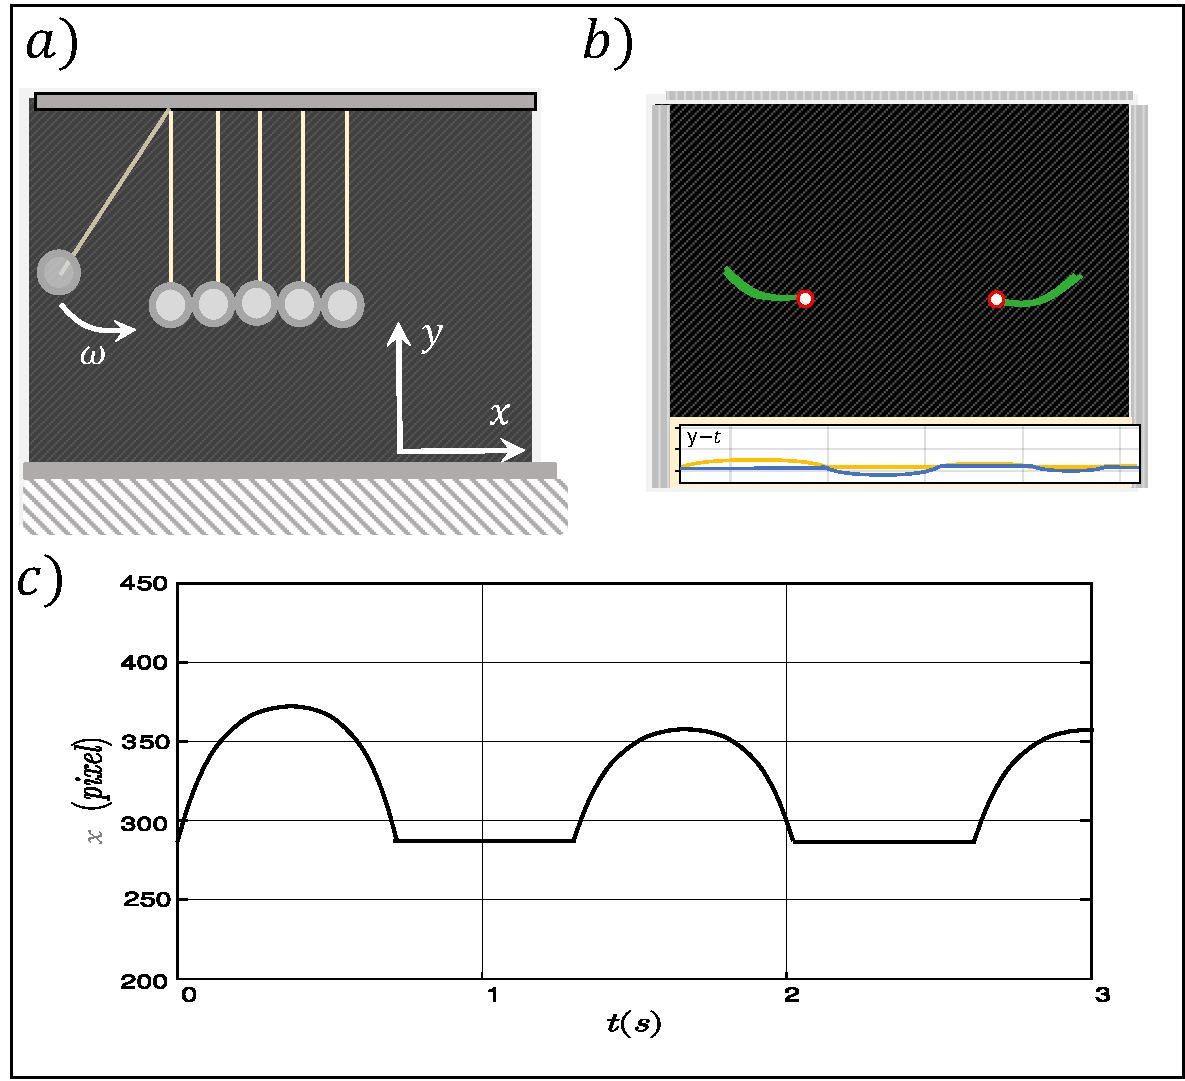
\includegraphics[width=12cm]{figures/Newtons_Cradle.pdf}
    \caption{The setup of the Newtons Cradle experiment. A spherical mass $m$ makes an angular motion with angular velocity $\omega$. At the moment of impact, the momentum (and energy) is transferred to the next sphere. The final sphere will have an lower final energy, thus the amplitude of the cradle will decrease. The Lumenera Li255C captures the motion of the outer spheres. The tracked trajectories are in shown b), the x-position is shown in c).}
    \label{Figure: Newtons cradle setup}
\end{figure}

% \section{Indeling dagdelen}

% \subsection{Dagdeel 1 (Verkenning)}
% Tijdens dit dagdeel wordt de basis gelegd voor de hardware en software door deze te verkennen en introducerende experimenten uit te voeren. Meestal begint de assistent dit dagdeel met een presentatie of een korte introductie over wat het experiment (bio)mechanica inhoudt. Er kan voor gekozen worden om de verkenning van de camera en driver (sectie 2 in de handleiding) samen te doen of de student dit zelfstandig te laten lezen. 

% \subsubsection{Opdracht 1}
% Tijdens dit deel moet worden gekeken naar de camera, lens en het programma LuCam Capture. Bij opdracht 1 is het de bedoeling de student kennis te laten maken met de camera, beugel en software. Ook wordt met behulp van een kalibratiepaneel het beeld gekalibreerd. Het paneel wordt belicht met theaterlampen om zo de zoom en focus goed in te stellen. Er wordt als laatste gevraagd naar de kleinste en grootste afstand vanaf de camera waar het paneel nog goed in focus is. Theoretisch gezien is het lastig om te bepalen wat 'goed in focus' is, omdat dit afhangt van meerdere factoren. De depth of field wordt gegeven door,
% \begin{align*}
% DoF \approx \frac{2u^2Nc}{f^2}
% \end{align*}
% waarbij $u$ de afstand tot het object, $N$ de $f$-number, $f$ de focal length en $c$ de circle of confusion. De circle of confusion hangt af van een aantal variabelen: de grootte van sensor, hoe groot het uitendelijke plaatje wordt afgebeeld enz. We nemen voor nu een circle of concfusion van $c=0.008$mm aan. Zie figuur \ref{fig:dof} voor hoe de verschillende factoren zich met elkaar verhouden.\\ Laten we een voorbeeld doen: Het kalibratiepaneel staat op een afstand van 2m. We proberen altijd een zo groot mogelijke sluiter (aperture) te gebruiken, in dit geval $f/1.4 \to N=1.4$. De circle of confusion was eerder gegeven $c=0.008$. Voor de focal length nemen we de kleinste focal length (dus zo ver mogelijk uitgezoomd), $f=11.5$mm. Dit geeft ons een $DoF\approx 677$mm. De kleinste afstand die nog goed in focus is, is dan $DoF_{\text{near limit}}=u-\frac{DoF}{2}=1.662$m en de grootste afstand is $DoF_{\text{far limit}}=u+\frac{DoF}{2}=2.339$m. Merk op dat de depth of field schaalt als het kwadraat van de afstand $DoF \sim u^2$, dus een kleinere afstand kiezen kan de depth of field significant verminderen.
% De ondergrens van de focus van de lens ligt rond een meter, en in principe zit er geen bovengrens aan de grootste afstand. Let wel op dat de nauwkeurigheid van de data onder andere afhankelijk is van de afstand tot het object, dus dit betekent dat je de camera zo dicht mogelijk wilt hebben. De uitdaging bij deze opdracht is het bepalen van de juiste focus. Dit kan lastig zijn maar belangrijk is om te zien of de grens tussen witte en zwarte vlakken niet wazig is. Door de depth of field is er een bereik aan focussen die 'goed' zijn, en meestal lijdt de kwaliteit er niet veel onder zolang het object binnen dit bereik ligt. Om vertekening van de beelden te voorkomen moet de voorkant van de lens goed parallel staan aan het objectvlak en dient de camera goed horizontaal of verticaal te staan.

% \begin{figure}
%     \centering
%     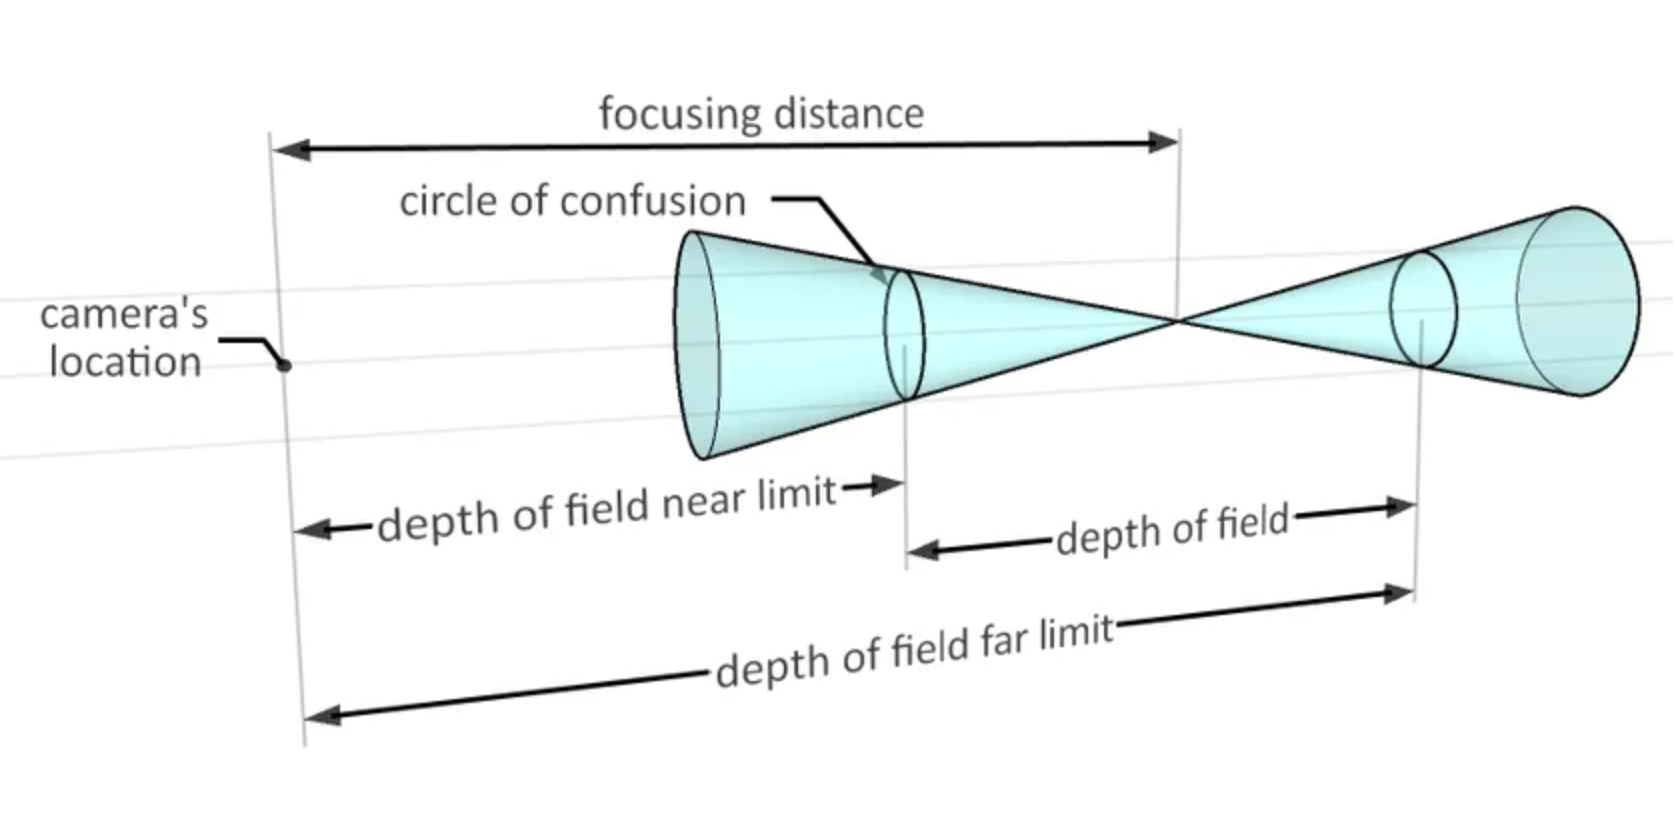
\includegraphics[width=\textwidth]{figures/dof.png}
%     \caption{Afgebeeld hoe lichtstralen vanaf de focus lopen. Hier is ook te zien hoe de depth of field afhangt van de circle of confusion. Een grotere circle of confusion betekent meestal ook een grotere depth of field.}
%     \label{fig:dof}
% \end{figure}

% \subsubsection{Opdracht 2}
% In deze opdracht wordt de software verkend en starten we eerst met TroublePix. Dit wordt uitgebreid in de handleiding uitgelegd en er kan hier weer gekozen worden om de student dit zelfstandig te laten lezen, of anders de video op Canvas te laten bekijken (er is nog geen video bij het schrijven van deze handleiding). Hierna volgt opdracht 2, in deze opdracht wordt de student aan het denken gezet over de bandbreedte tijdens het filmen. De bandbreedte (informatie per seconde, in dit geval bits of bytes per seconde) wordt gegeven door
% \begin{equation}\label{eq:1}
%     \text{bandwidth} = \text{resolution} \times \text{frame rate} \times \text{color depth}
% \end{equation}
% waarbij de resolution wordt berekend door het product van de verticale en horizontale pixels. Color depth, of kleurendiepte, is een maat voor de hoeveelheid kleuren die een pixel kan aannemen. Voor dit experiment wordt er 8-bit grayscale gebruikt (8-bit zwart-wit), wat betekent dat er $2^8=256$ zwart-wit tinten beschikbaar zijn. We zullen tijdens dit experiment zwart-wit gebruiken omdat kleur (in TroublePix 12-bit) in de meeste gevallen geen toegevoegde waarde heeft. De bandbreedte wordt ook gelimiteerd door de gebruikte dataverbinding, in ons geval het USB 3.0 protocol. Een voorbeeld voor USB 3.0: De maximale theoretische overdrachtssnelheid die USB 3.0 kan leveren is 5 Gbps (5 Gigabit per seconde = 625 MegaByte per seconde, b = bit en B = Byte). Als we dit vergelijken met de bandbreedte van de video met de best mogelijke (maximale resolutie, beste kleurendiepte en hoogste frame rate) die de camera kan leveren komen we uit op een bandbreedte van $2048 \times 1088 \times 170 \times 12 = 4,55$ Gbps = 568,75 MBps. \\Dit betekent dat een filmpje van een aantal seconde al snel gigabytes aan opslag kan vullen. Omdat we de kleurendiepte constant houden is de bandbreedte een strijd tussen de resolutie en de frame rate, dus als je bijvoorbeeld een filmpje wilt opnemen met een hogere frame rate moet je een lagere resolutie nemen. Een andere resolutie kiezen kan je op twee manieren doen: je kan uit de lijst van resoluties de kiezen of je kan de Region Of Interest (ROI) aanpassen, waardoor je in principe een custom resolutie maakt. Bij opdracht (a) wordt er gevraagd naar de maximale frame rate bij maximale resolutie, dit is voor 8-bit ongeveer 250 fps. De student zal hierachter moeten komen door daadwerkelijk het filmpje te maken, omdat de berekeningen die we hi er doen kunnen afwijken van de praktijk. Het is mogelijk dat de frame rate significant kan afwijken (in de tientallen procenten) als de camera erg warm is of als de camera is aangesloten aan een USB 2.0 poort. De camera kan in portrait (langer verticaal dan horizontaal) en landscape (langer horizontaal dan verticaal) worden gepositioneerd. Voor een object wat valt is het handiger om het in portrait te zetten, omdat de beweging van een vallend object alleen maar in de hoogte (dus verticaal) gebeurt. Bij (c) wordt er gevraagd hoe we nog een hogere frame rate kunnen halen. Zoals eerder genoemd is de bandbreedte afhankelijk van de frame rate en resolutie. Omdat we werken met de maximale resolutie, kunnen we een kleinere resolutie nemen en hiervan de ROI aanpassen om zo een hogere frame rate te krijgen.

% \subsubsection{Opdracht 3}
% Dit is de eerste opdracht waarbij alle kennis over hardware en software wordt toegepast bij een experiment. De studenten zullen met deze opdracht de valversnelling $g$ bepalen met behulp van een slinger. Hiervoor gebruiken we een model van een simpele harmonische oscillator, in plaats van een gedempte oscillator (kan alsnog gebruikt worden als verdiepende opdracht). De reden dat we geen gedempte oscillator gebruiken is omdat het filmpje wat wordt opgenomen maar een paar oscillaties zal bevatten. Bij (a) wordt er gevraagd waarom we de luchtweerstand kunnen verwaarlozen en als hint wordt gegeven dat de luchtweerstand evenredig is met het kwadraat van de snelheid. We mogen dit doen om twee redenen: als eerste, we kijken maar naar een paar oscillaties, dus dat betekent dat de amplitude van ons signaal nauwelijks afneemt over deze tijd. Als tweede, we mogen luchtweerstand verwaarlozen voor dezelfde reden dat ons model evenredig is aan een sinus, want we kijken naar kleine hoeken waar de snelheid relatief klein is. Nu is het aan de student om de opstelling te bouwen en de meting te doen. Als het goed is staat de camera al klaar en moet alleen de slinger klaargezet worden. De slinger zelf kan belicht worden met theaterlampen of er kan een LED lichtje worden opgehangen. Vervolgens moeten de studenten met TroublePix de best mogelijke instellingen vinden om uiteindelijk een frame rate van ongeveer 300 fps te behalen. De makkelijkste instelling is de sluitertijd, die mag maximaal $\frac{1}{300}$s zijn. Vervolgens kan je met de hoogste resolutie en juiste ROI kijken of je 300 fps kan bereiken, zo niet pas dan eerst de resolutie en dan de ROI aan. Bij het bouwen van de opstelling moet goed gelet worden op een aantal dingen:

% \begin{itemize}
%     \item Zorg ervoor dat de camera loodrecht staat op het vlak waarin de slinger oscilleert, als dit niet het geval is zal de beweging niet mooi sinusoidaal lijken te zijn in de video.
%     \item Ook moet gelet worden op dat de camera niet te ver naast of boven de slinger staat
%     \item Als het aangrijppunt niet 'perfect' is krijg je een variabele lengte van de slinger wat invloed heeft op de bepaalde waarde van $g$.
%     \item Ook zal de waarde afwijken als de lengte van de slinger onjuist is bepaald.
% \end{itemize}

% Dit zijn tevens ook een van de redenen dat de theoretische waarde kan afwijken van de experimentele waarde. We zoeken bij (c) vooral naar het onjuist positioneren van de camera.

% \subsection{Dagdeel 2}
% Het tweede dagdeel zal vooral bedoeld zijn voor het verkennen en kiezen van een keuze-experiment, en het schrijven van een werkplan. Het kan zijn dat de verkenning van dagdeel 1 uitloopt tot dit dagdeel, maar deze uitloop moet tot een minimum gehouden worden omdat bij dit experiment de uitvoering van de experimenten vrij lang kan duren. Er kan gekozen worden voor een biomechanisch of een klassiek mechanisch experiment. Belangrijk is dat de studenten tijdens dit dagdeel al goed duidelijk hebben wat ze willen bepalen, of hier een model/theorie voor is en of het experiment haalbaar is, bespreek dit ook met de stafleden.

% Het is vooral bij dit experiment belangrijk dat de studenten goed nadenken over hun keuze-experiment voordat ze deze gaan uitvoeren. Dit betekent dat het werkplan zoveel mogelijk een complete theorie en methode moet bevatten. Het is op zich niet erg als deze niet helemaal correct of compleet zijn, maar pas wel op dat de student niet in tijdsnood komt omdat het niet duidelijk is wat er gedaan moet worden.

% \subsection{Dagdeel 3}
% Het eerste dagdeel waar de studenten zullen beginnen met hun keuze-experimenten. Dit dagdeel begint dan met een korte introductie en het bespreken van de werkplannen. In dit dagdeel zullen de koppels studenten de werkplannen laten presenteren onder begeleiden van de assistent. De presentaties worden dan van feedback voorzien door de assistent en de medestudenten. Het is sterk aangeraden dat de studenten de opstelling bouwen, 1 meetserie doen en deze vervolgens helemaal gaan analyseren. Zo hebben ze een keer de stappen in hun werkplan doorgewerkt en gecontroleerd of hun theorie en methode kloppen.

% \subsection{Dagdeel 4 en verder}
% In de komende dagdelen zullen studenten verder werken aan hun experiment en de data analyseren die ze tijdens deze dagdelen hebben verkregen. Het zou voor de studenten die een biomechanisch experiment doen erg nuttig zijn om bronnen te vinden waarmee ze hun data kunnen vergelijken. Het zou optimaal zijn als dit al is uitgezocht in het werkplan, maar het is ook mogelijk om dit in de later dagdelen uit te zoeken mits daar tijd voor is. 
\end{document}
